\chapter{Theory}\label{theory_part}
This chapter goes through the various techniques used in image processing. This section is a general description, while chapter \ref{implementation} will describe how they were used for this specific project.

\section{A general framework for image processing}
During this project image processing has been used to achieve the output needed. Some techniques were used to remove noise from the picture, so that the important parts get all the focus, while others were used to make the important parts more clear or to track specific objects. Image processing can be described as an umbrella term. \citep{ip_book} writes that Image processing comes from the general field of signal processing, and that it covers ways to segment objects of interest on a digital image. This is achieved by using multiple steps. It should be noted, however, that the order of the steps sometimes changes, and there might be more focus on some than others. Still, this is a general framework that can be used as a good starting point (based on \citep{ip_book}). Figure \ref{fig:ip_framework} illustrates a common framework when working with image processing.

%\textbf{Image Acquisition}
%Before anything can be processed, data needs to be captured, typically using a camera. This step is all about the setup, as well as the environment, setting, lighting and so on.

%\textbf{Pre-processing}
%Here the initial arrangement is completed, e.g. converting the image from color to grayscale.

%\textbf{Segmentation}
%To be able to work with a specific object, for instance a hand, it needs to be separated from the rest of the picture. This is done using segmentation to remove noise and background elements, so that only the object of interest is seen. Thresholding is often applied to make the object stand out, i.e. make the object appear white and the background black.

%\textbf{Representation}
%The object needs to be represented in an intuitive manner.

%\textbf{Classification}
%For the system to actually know if an object is a hand or not, it has to do some features extraction and classifications to compare the data to some predefined database. This can be done with template matching and BLOB classification.

\begin{figure}[htbp]
\centering
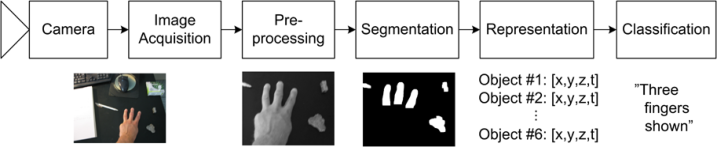
\includegraphics[width=1.00\textwidth]{Pictures/Theory/imageProcessing_steps.png}
\caption{Image Processing framework, from \citep{ip_book}.}
\label{fig:ip_framework}
\end{figure}

%% Maybe a little too blabla and too long sentences - Gustav %%
%% I moved a paragraph to the begining of the section and changed some things. But I'm still not sure if the above part is useful, as we will be describing everything again... - Marta %%

The combination of these different techniques makes it possible to get a functional program, but before using them, it is necessary to know how they work. The next sections will explain the different techniques used and also why and how they were implemented in the project. 

\section{The digital image}
Behind the image acquisition applications often used in our daily life, such as cameras, or the image manipulation programs like \href{http://rsbweb.nih.gov/ij/}{ImageJ}, several different computations are needed. Even when the users do not need to understand the physics behind the light, the electronics inside their machines and the data structure on the programs. To be able to get some useful information from images and use it for further purposes it is necessary to have a previous knowledge. Figure \ref{fig:ip_ColoredToGrayscaleToBinary} shows what this chapter is all about; working with color, grayscale or binary images, and the different attributes of each type.

\begin{figure}[htbp]
\centering
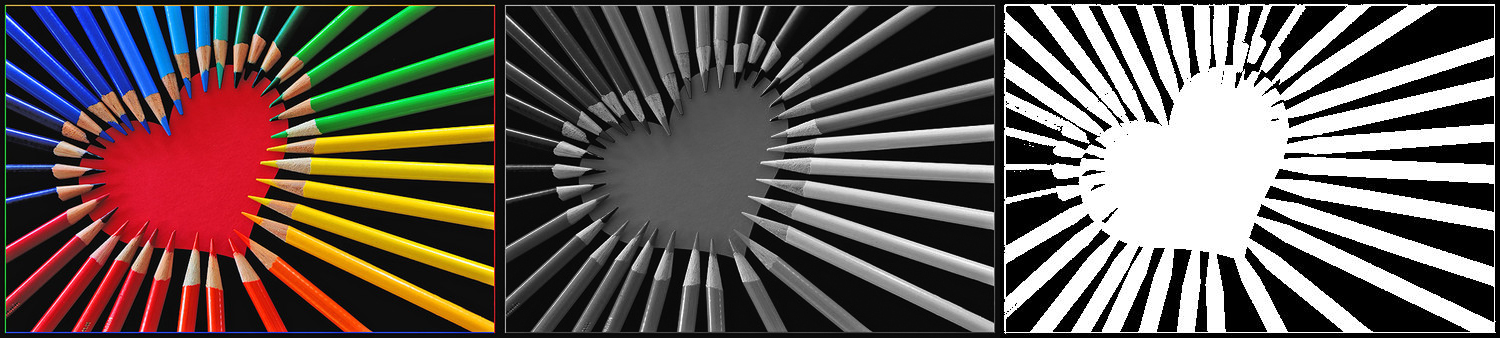
\includegraphics[width=1.00\textwidth]{Pictures/Theory/ColoredToGrayscaleToBinary.jpg}
\caption{Image illustrating a conversion from a colored image to grayscale and finally to binary (only black and white).}
\label{fig:ip_ColoredToGrayscaleToBinary}
\end{figure}

\subsection{Pixels}
When a digital camera takes a picture, it uses an image sensor consisting of an array of interconnected cells. All cells hold a filter, a sensor and an output. When light hits the cells, the energy is converted into a digital number via an analog-to-digital converter (ADC). This value is denoted a \textit{pixel} and describes how bright a specific part of the image should be \citep{ip_book}.

\subsection{8-bit image and grayscale images}
In an 8-bit image, the 8-bit prefix describes the \textit{bit depth} of the image. The bit depth tells us about the amount of information that can be stored in a single pixel.

An image with a single channel of information for each pixel in the X and Y axis is typically a grayscale image, since each pixel is limited to information about a single hue. The hue defines how pure and vivid a color is \citep{visual_story}. The information stored in each pixel is the brightness of the particular pixel. 8 bit evaluates to $2^8$ different states, meaning that a single 8-bit pixel can display 256 different levels of intensity, or in the case of a zero-based computer system, 0-255 (see figure \ref{fig:ip_grayscale}). An 8-bit image is a widely-used format for images, but it is also possible to create images with more depth and with more information for each individual pixel. Examples of that are images in 16 and 32 bits. A 16-bit depth is equal to $2^{16}$ different states, which means that each pixel can hold any one of 65,536 different shades of gray. Simultaneously, a 32-bit depth is equal to $2^{32}$, which gives 4,294,967,296 different shades of gray.

\begin{figure}[htbp]
\centering
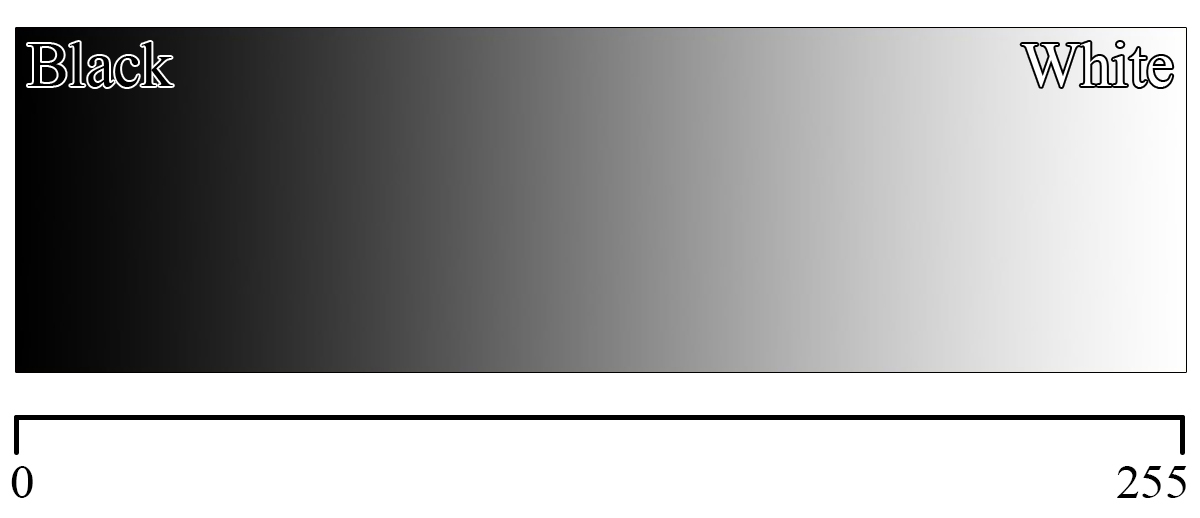
\includegraphics[width=0.7\textwidth]{Pictures/Theory/Grayscale.jpg}
\caption{Image illustrating the 256 different gradients of an 8 bit picture.}
\label{fig:ip_grayscale}
\end{figure}
 
\subsection{Indexing an image}
When working with images on a computer and performing image processing, one often has to look at the individual pixels within an image.

Working with pixels in a image is like working with a coordinate system. Starting in the top-left corner is (0,0). Going to the right, the X value increases; going down, the Y value increases. A single pixel can be described as a coordinate, e.g. on figure \ref{fig:ip_IndexingAPicture} the pixel (1192,666) is the bottom-most corner to the right.

\begin{figure}[htbp]
\centering
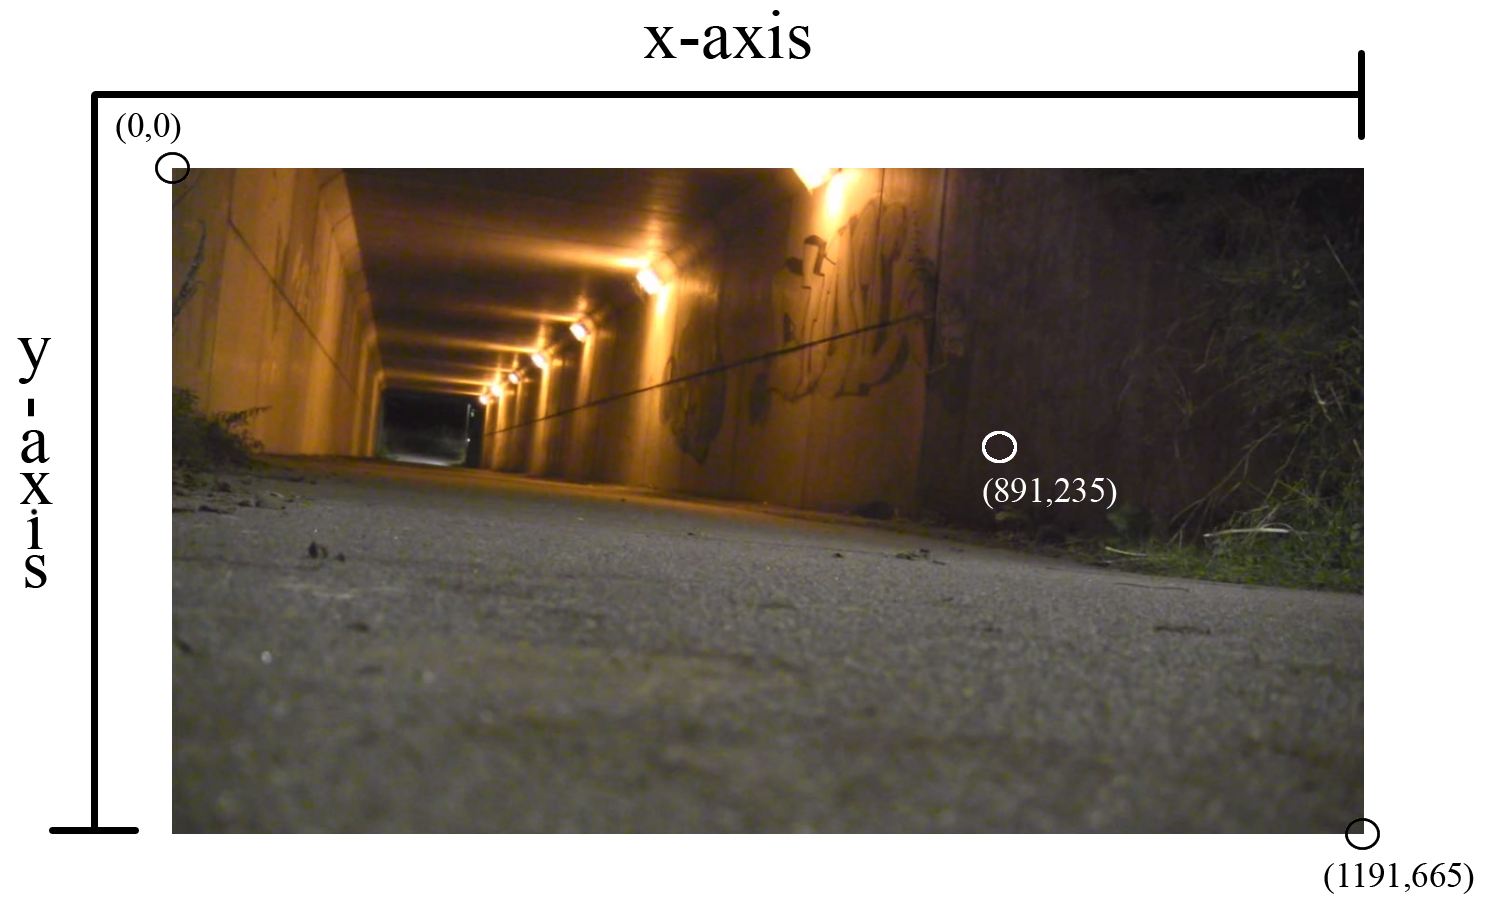
\includegraphics[width=1.00\textwidth]{Pictures/Theory/IndexingAPicture}
\caption{The pixel values are stored in a coordinate system. Note that Y goes down and not up.}
\label{fig:ip_IndexingAPicture}
\end{figure}

\textbf{[WE NEED TO CHANGE THE PIC!!!!!!!! TOO DARK!!! ... ]}

In OpenCV, images are stored in a matrix (see figure \ref{fig:opencv_matrix}). The size of the matrix holding the pixel values of the X and Y axis is as wide as the proportions of the image, therefore, when an image with a resolution of \textit{1024*1024} pixels is loaded, the highest coordinate assigned to pixels in the the matrix is (1023,1023).

\textbf{[WE NEED TO DESCRIBE OPENCV MATRICES BETTER!!! ... Max?]}

\begin{figure}[htbp]
\centering
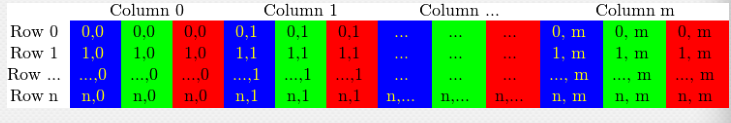
\includegraphics[width=1.00\textwidth]{Pictures/Theory/opencv_matrix}
\caption{OpenCV stores the pixel values in a matrix system. Picture from \citep{opencv}.}
\label{fig:opencv_matrix}
\end{figure} 

\subsection{Working with coloured images}
Now that a basic knowledge regarding images has been established, the next step into using images in calculations is to understand the basics of a colored image.

There are several formats for handling color images. In this report we will only decribe RGB, since this is the only format we will encounter. The main difference when talking about colored and grayscale images, is that colored images have 3 channels, compared to the single channel in grayscale images. Each of the three channels holds the value of its specific color for each pixel in relation to red, blue or green, which are the primary colors our eyes are sensitive to. Therefore, a colored image doesn't describe the intensity of a specific color, but the amount of the red, green and blue the pixels contain. In addition, equal amounts of red, green and blue will produce a gradient of grey. A pixel with the color channels values of 255 produces a white pixel, and a pixel with the color channels values of 0 will produce a black pixel. This phenomenon can be easily understand by looking to figure \ref{fig:ip_ColorWheel}, where the additive color system of wavelengths illustrates the colors' formation.

Knowing the specific values of the red, green and blue channels within an image gives the user a great advantage, especially when performing image manipulations in programming. To exclude a specific color in a mathematical operation, such as red, it's necessary to use thresholding to segment the pixels depending on values of the red channel (this will be described in \ref{sec:Thresholding}). The outcome in that case would be a picture with a limited/controlled amount of red.

\begin{figure}[htbp]
\centering
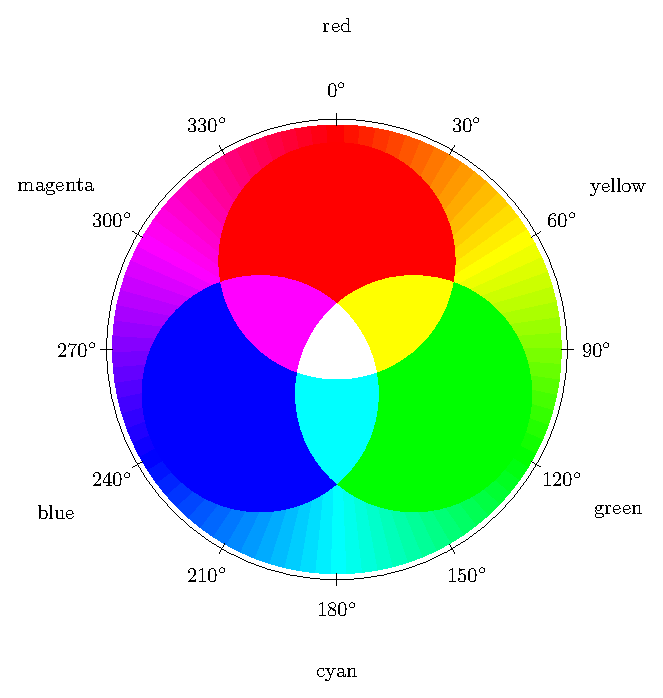
\includegraphics[width=0.50\textwidth]{Pictures/Theory/RGBColor.pdf}
\caption{Image illustrating the making of colors - \citep{colorMixing}}
\label{fig:ip_ColorWheel}
\end{figure} 

\subsection{Binary Images}
In comparison to the above-mentioned where images are defined by bit depth and pixel information, binary pictures are represented by two colors only in form of black and white. This often correlates to using a threshold. Binary pictures are less resource demanding when performing mathematical operations as each pixel only can take one of two values.

Using the tool correctly, it is possible to adjust the input so that only usable pixel information remains in the picture. However, this should be carefully done, as the input can be easily over- and undersegmentated. Threshold would be developed further more on next sections.

\section{Histograms}
A commonly-used tool when working with digital images are histograms. Essentially a histogram provides data distribution, which is an easy way to get an overview of the frequency of events. An image histogram is a graphical representation of the pixel values. This is used to show whether an image is too dark or too bright, as well as how good the contrast is \citep{ip_book}. Figure \ref{fig:SimpleThreshold} shows a histogram with pixel values from 0-255, which cover the entire graphic as each pixel value has a bin. The more often a specific pixel value is present on the image, the taller the bin will be. The image shows a histogram with a high concentration of bins near the edges (0 and 255). This means that the picture is mostly black and white with few nuances in-between.

\begin{figure}[htbp] \centering
\begin{minipage}[b]{0.45\textwidth} \centering
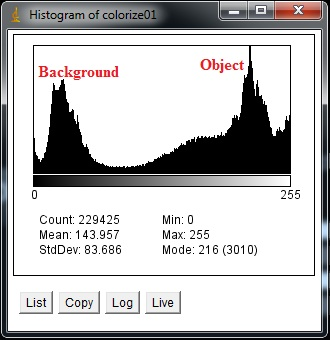
\includegraphics[width=1.00\textwidth]{Pictures/Theory/SimpleThresholdPicture} % Venstre billede
\end{minipage} \hfill
\begin{minipage}[b]{0.45\textwidth} \centering
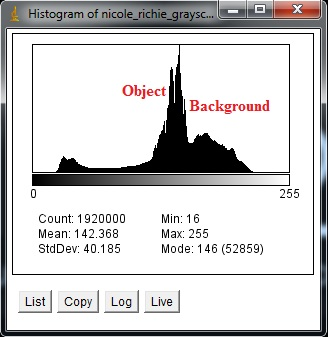
\includegraphics[width=1.00\textwidth]{Pictures/Theory/ComplicatedThresholdPicture} % Højre billede
\end{minipage} \\ % Captions og labels
%\end{figure}
\begin{minipage}[t]{0.45\textwidth}
\caption{Ideal histogram with two "mountains".} % Venstre caption og label
\label{fig:SimpleThreshold}
\end{minipage} \hfill
\begin{minipage}[t]{0.45\textwidth}
\caption{Problematic histogram.} % Højre caption og label
\label{fig:ComplicatedThreshold}
\end{minipage}
\end{figure}

As said before, histograms can also be used to describe the contrast in an image. The contrast is a measure of the difference of intensity levels between the dark and light areas on the picture \citep{histogram}. This means that a histogram with broad values, will represent an image with good contrast. On the other hand, if the histogram is very narrow, the contrast in the image is smaller, and it will appear more flat and dull (see figure \ref{fig:histogram_contrast}).

\begin{figure}[htbp]
\centering
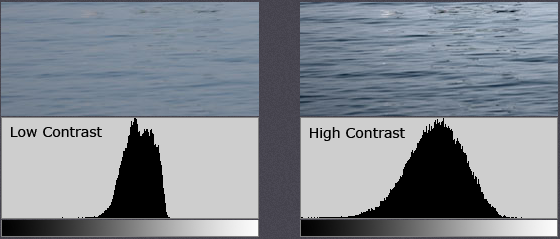
\includegraphics[width=0.80\textwidth]{Pictures/Theory/hisogram_contrast.png}
\caption{Histograms can be used to describe the contrast in an image. Picture from \citep{histogram}.}
\label{fig:histogram_contrast}
\end{figure}

\section{Thresholding}\label{sec:Thresholding}
Thresholding is one of the most fundamental operations when working with images. It is performed to transform a picture to binary; i.e. either black, which relates to the pixel value of 0 or white, which relates to the pixel value of 255. Making an image binary means to show the image in only black and white pixel values.

This is useful in programs where you need to find silhouettes, such as tracking a person, where smaller details are not important.

To determine which pixels should be completely black and which pixels should be completely white a fixed \textit{thresholding value} is required. Using a metaphor, the \textit{threshold value} can be compared to a gatekeeper that lets everyone who is 18 years old or older inside the club, but denies access to people who are 17 or younger. Using this analogy, pixels that are "old" (bright) enough are let in, while "younger" pixels (dark) are denied. The value used to classify which persons (or pixels) can pass and which have to stay out, have to be decided by the gatekeeper (or the programmer, in our case).

In practice this means that pixels with values greater than a threshold is set to TRUE (or white), which typically is 255 when talking in bytes. On the other hand, if a pixel is less than the threshold value, it is set to FALSE (black) or 0. To sum this up, the formula for making a threshold is shown in equation \ref{threshold}.
\begin{equation}
  \begin{aligned}
  	\text{if } f(x,y)\leq T \quad \text{then } g(x,y)&= 0 \\
  	\text{if } f(x,y)>T \quad \text{then } g(x,y)&= 255
	\label{threshold}  
  \end{aligned} 
\end{equation}
Where $T$ is the threshold value, $f(x,y)$ is the input pixel and $g(x,y)$ is the output pixel. 

When setting the thresholding value it is important to think about what is wanted regarding the output. The effectiveness of the \textit{threshold value} will differ from image to image, depending on the contrast between the object and the background. If the background and the object are very different in color and/or contrast, it will be easy to distinguish them and choose an effective \textit{threshold value}. However, if the object and background are very similar, it will be hard to choose a value to separate them properly. At that point it will be necessary to choose between losing information associated to the object of interest or to gather some background noise, to preserve it. Pictures \ref{fig:SimpleThreshold} and \ref{fig:ComplicatedThreshold} show the \textit{threshold value} used on the images \ref{fig:SimpleThresholdAfter} and \ref{fig:ComplicatedThresholdAfter}. Looking to the histograms, it is easy to tell that the leftmost is more ideal to threshold because the object and background are very different. That is shown graphically with two "mountains" in the histogram (see picture \ref{fig:SimpleThreshold}), also called a \textbf{bi-modal histogram} \citep{ip_book}. The effect of a good threshold value can be seen on picture \ref{fig:SimpleThresholdAfter}, where the output gives a clear outline of the silhouette of the woman. On the other hand, the histogram to the right does not have two clear mountains, but a big one and two smaller. This means that the color values are distributed more equally and therefore, it will be hard to define a good threshold value. The result in this case is a poor silhouette of a woman (see picture \ref{fig:ComplicatedThresholdAfter}), due to the fact that the background and the object have similar colors.

%Looking at picture \ref{fig:SimpleThresholdAfter} will show that the picture with the leftmost histogram, figure \ref{fig:SimpleThreshold}, gives a clear outline of the silhouette of a woman after the thresholding value is applied. However, looking at figure \ref{fig:ComplicatedThresholdAfter} shows that the picture with the rightmost histogram, figure \ref{fig:ComplicatedThreshold}, produces a poor silhouette of a woman, due to the fact that the background and the object has very similar colors. 

\begin{figure}[htbp] \centering
\begin{minipage}[b]{0.45\textwidth} \centering
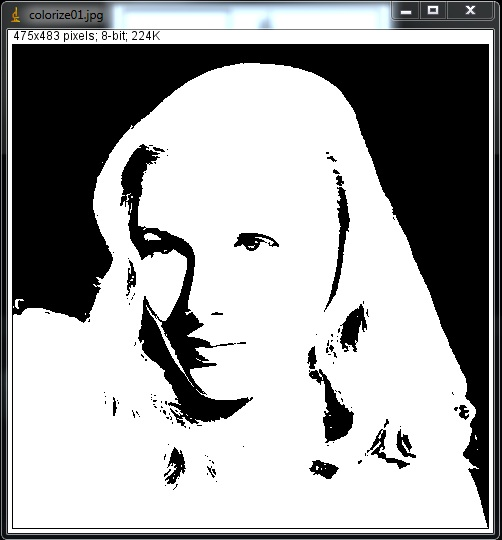
\includegraphics[width=1.00\textwidth]{Pictures/Theory/SimpleThresholdAfter} % Venstre billede
\end{minipage} \hfill
\begin{minipage}[b]{0.45\textwidth} \centering
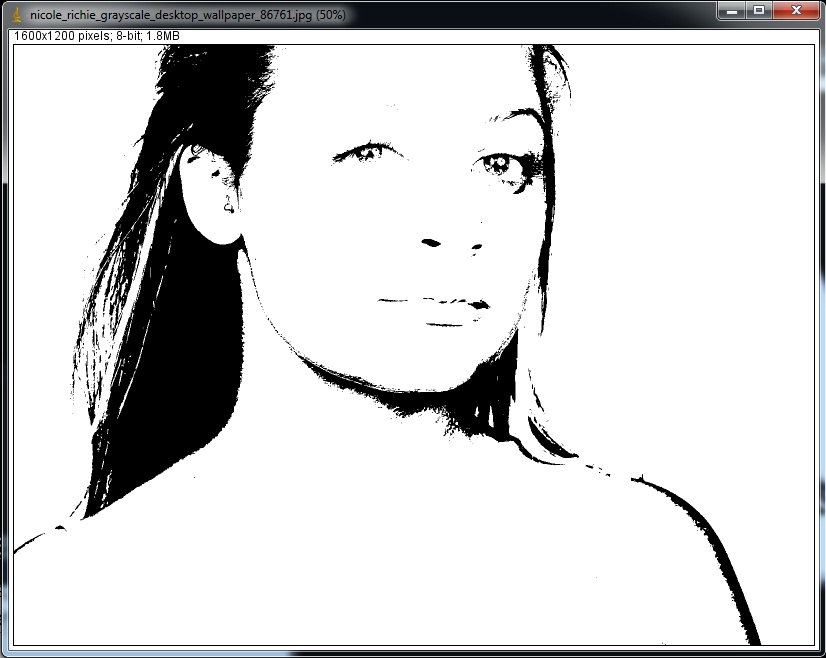
\includegraphics[width=1.00\textwidth]{Pictures/Theory/ComplicatedThresholdAfter} % Højre billede
\end{minipage} \\ % Captions og labels
\begin{minipage}[t]{0.45\textwidth}
\caption{Good silhouette after thresholding.} % Venstre caption og label
\label{fig:SimpleThresholdAfter}
\end{minipage} \hfill
\begin{minipage}[t]{0.45\textwidth}
\caption{Bad silhouette after thresholding.} % Højre caption og label
\label{fig:ComplicatedThresholdAfter}
\end{minipage}
\end{figure}
 
This proves the point that finding a functional thresholding value is not always straightforward. As for finding a silhouette it is of great help to make a clear transition from the object and the background.

\section{Morphology}
Morphology is a collection of operations used to analyze and process structures. Although these techniques are commonly used on binary images, it is possible to apply them to grayscale images as well. The processes related to morphology on binary images are often used to remove noise produced by thresholding an image, as well as defining the contours of the objects in order to achieve a proper BLOB analysis \citep{ip_book}.

Morphology is a a part of neighbourhood processing. Whereas point processing is about each individual point (pixel), neighbourhood processing is about taking a pixel and its surrounding neighbours, i.e. to get an average pixel value. For this purpose a kernel is used, as shown in figure \ref{fig:kernel}. %is the last sentence correct there?

\begin{figure}[htbp]
\centering
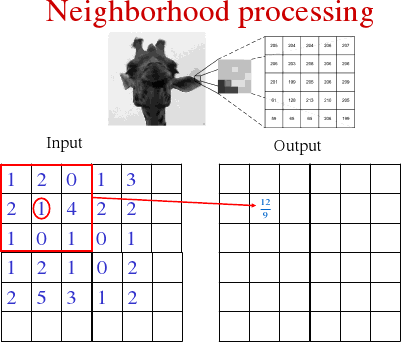
\includegraphics[width=0.7\textwidth]{Pictures/Theory/kernel}
\caption{Neighbourhood processing uses a kernel. Image from \citep{ip_book}.}
\label{fig:kernel}
\end{figure}

\subsubsection{Hit and fit}
Whenever one decides to apply a structured element and \textit{hit} the pixels, what happens is that the function will calculate the value of the output pixel by comparing the values of the pixels on the input image and the kernel. A kernel is a grid containing weighted values. These values are either 1 or 0 if used on a binary pixel. Depending on these values and the images pixel values different output occur.

The process of hitting the pixels starts positioning the kernel on the corner of the image so that it operates on one pixel at a time. If one of the pixels inside the kernel are '1' where the kernel is '1' as well, then it is said to hit. This means that the pixel in the center of the kernel will become a '1' (white) in the output. If none of the pixels inside the kernel "hits", then the pixel in the middle of the kernel becomes a '0' (black) in the output.

\begin{figure}[htbp]
\centering
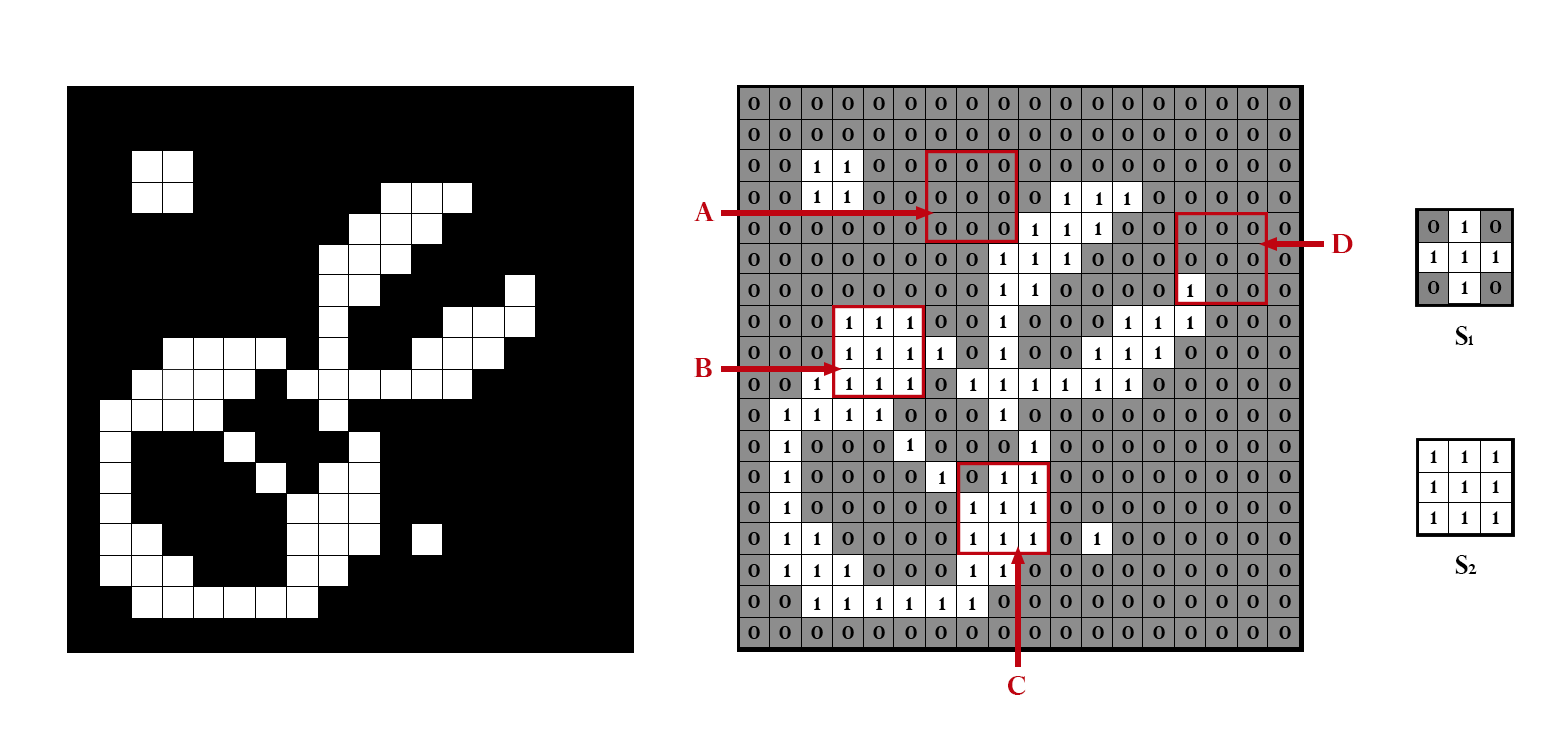
\includegraphics[width=1\textwidth]{Pictures/Theory/FitHitKernels.png}
\caption{Binary image and structuring elements.}
\label{fig:FitHit}
\end{figure}

On the contrary, to be able to \textit{fit} a pixel on the center of the structured element, every pixel's neighbour values have to be the same both on the kernel and the input image. If one of the pixels on the input image have a different value to the corresponding 1's of the kernel, the pixel in which the kernel is centred will be a '0' on the output image. On table \ref{tab:HitFitResults} figure \ref{fig:FitHit} has been represented with two different types of structuring elements.
\begin{table}[htbp]
\centering
\begin{tabular}{|c|c|c|c|}
\hline
 \:Position\: &SE &\:\:\:Hit\:\:\: &\:\:\:Fit\:\:\: \\\hline
 \hline
 A &$S_{1}$ &No &No\\\hline
 A &$S_{2}$ &No &No\\\hline
 B &$S_{1}$ &Yes &Yes\\\hline
 B &$S_{2}$ &Yes &Yes\\\hline
 C &$S_{1}$ &Yes &Yes\\\hline
 C &$S_{2}$ &Yes &No\\\hline
 D &$S_{1}$ &No &No\\\hline
 D &$S_{2}$ &No &No\\\hline
\end{tabular}
\caption{Results of hitting and fitting with two different structuring elements.}
\label{tab:HitFitResults}
\end{table}

\subsection{Dilation}
\textit{Dilation} is the process of applying the hit process to an entire image, and it refers to the expansion of an object on an image (see eq.\ref{Dilation1} for a mathematical definition). The result of this method implies filling small holes and merging objects. As mentioned before, the final effect on these objects will depend on the structured element (how big it is and which shape it has), this can be seen on figure \ref{fig:Dilation}. 
\begin{equation}
\begin{aligned}
{g(x, y)}={f(x,y)}\oplus{SE}
\label{Dilation1}
	\end{aligned}
\end{equation}
A small structured element applied several times will have the same effect as a big structured element passed once. This can be seen on eq. \ref{Dilation2} where dilating twice with the element {$SE_{1}$} has the same consequences on the object as dilating one time with {$SE_{2}$}, even though the only difference between those two kernels is that {$SE_{2}$} has a radius twice times bigger than the radius of {$SE_{1}$}.
\begin{equation}
\begin{aligned}
{f(x,y)}\oplus{SE_{2}} \approx ({f(x,y)}\oplus{SE_{1}})\oplus{SE_{1}}
\label{Dilation2}
	\end{aligned}
\end{equation}
%%%%%%%%%%%%%%%%%%%%%%%%% IMAGES WITH DILATIONS %%%%%%%%%%%%%%%%%%%%%%%%%%%%%%%%%%%%
\begin{figure}[htbp]
\centering
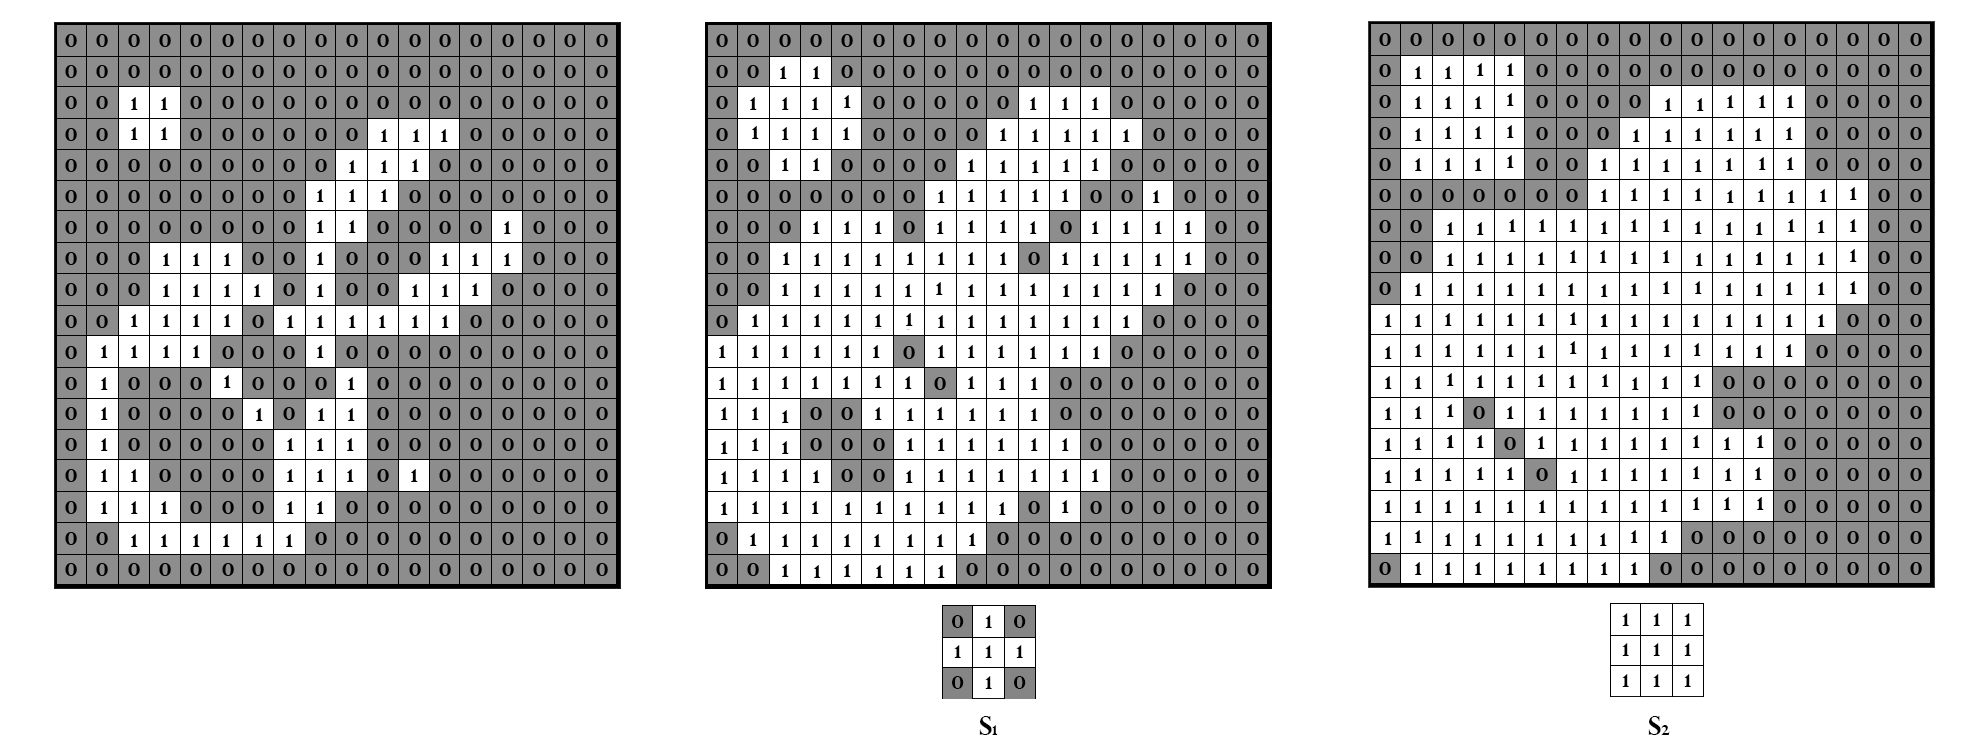
\includegraphics[width=1\textwidth]{Pictures/Theory/Dilation.png}
\caption{Dilation produced by two different structuring elements.}
\label{fig:Dilation}
\end{figure}

\subsection{Erosion}
\textit{Erosion} is the process of applying fit to an entire figure and refers to the reduction of the size of an object in an image (the mathematical definition is provided on eq. \ref{Erosion1}). As the fit method is applied, small objects will also disappear and larger objects will be break down into smaller ones. As it happens with dilation, the effects depend on the size and shape of the structured element.
\begin{equation}
\begin{aligned}
{g(x, y)}={f(x,y)}\ominus{SE}
\label{Erosion1}
	\end{aligned}
\end{equation}

%%%%%%%%%%%%%%%%%%%%%%%%% IMAGES WITH EROSIONS %%%%%%%%%%%%%%%%%%%%%%%%%%%%%%%%%%%%
\begin{figure}[htbp]
\centering
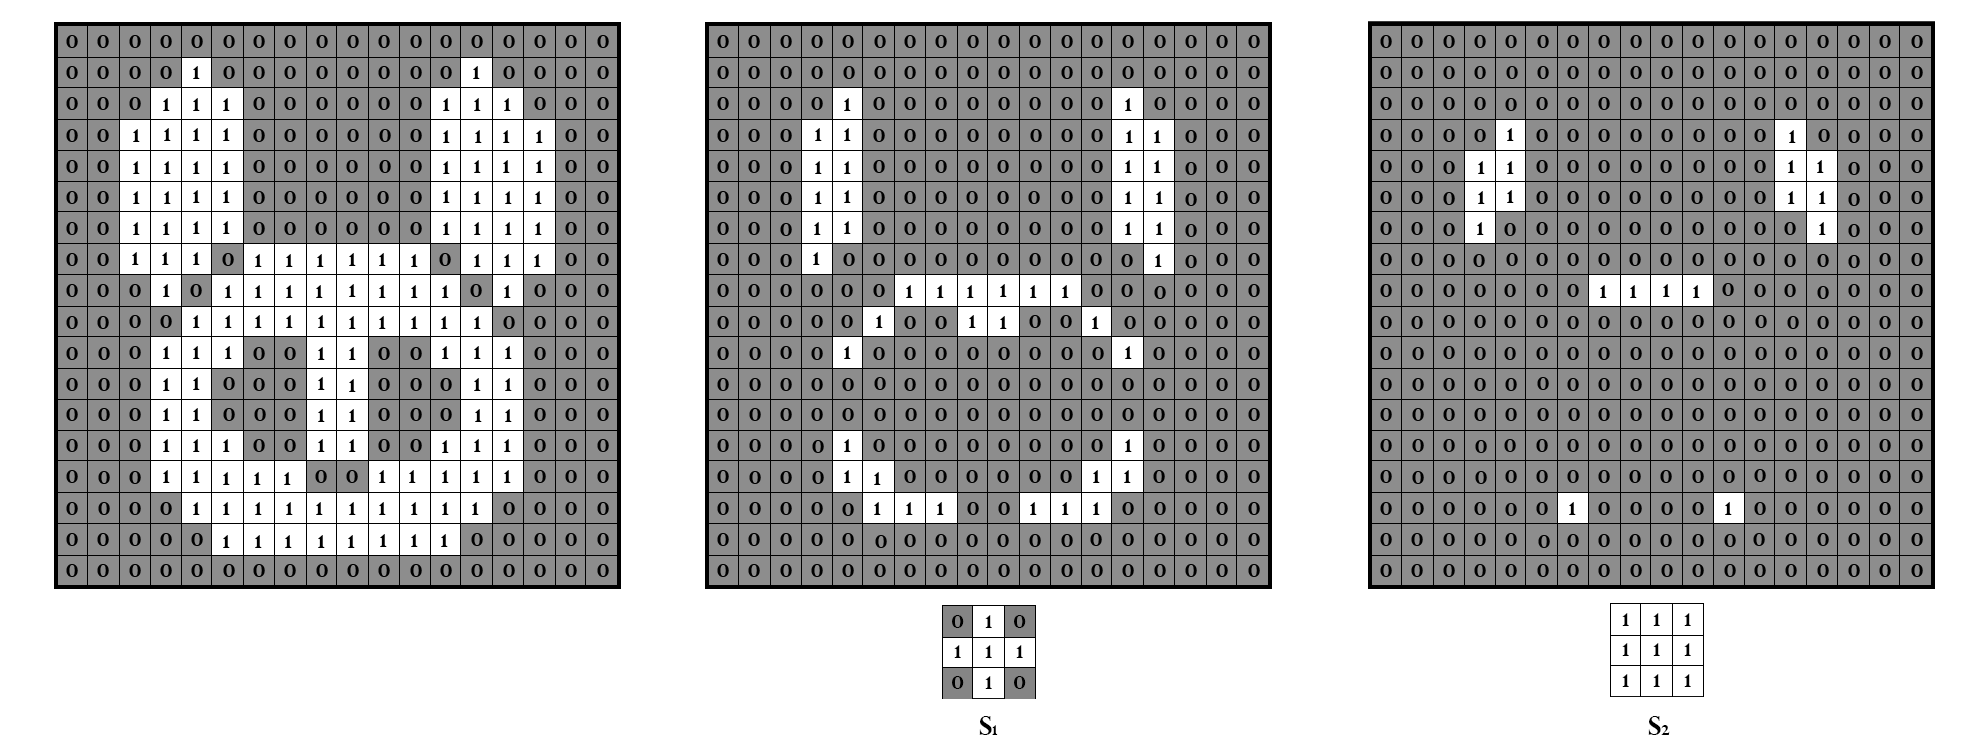
\includegraphics[width=1\textwidth]{Pictures/Theory/Erosion.png}
\caption{Erosion produced by two different structuring elements.}
\label{fig:Erosion}
\end{figure}

\subsection{Compound operations}
The term \textit{compound operations} refers to the combination of dilating and eroding objects on an image and can therefore imply the \textit{union} or \textit{intersection} of the objects, but also other operations like \textit{closing}, \textit{opening} or doing edge detection, also know as \textit{boundary detection}.
\subsubsection{Opening}
When \textit{eroding} images to erase small noise objects or split parts, it often occurs that the object of interest has decreased its size. The solution to this problem is to dilate the eroded image. This operation is denoted \textit{opening}, as shown in eq. \ref{Opening}.
\begin{equation}
\begin{aligned}
{g(x,y)}={f(x,y)}\circ{SE}=({f(x,y)}\ominus{SE})\oplus{SE}
\label{Opening}
	\end{aligned}
\end{equation}
The effect of opening can be seen on figure \ref{fig:Opening} where a circular kernel is applied to the image. Even though the object still maintains its original size, some information has been lost due to the effect of eroding and dilating the image, even if the same structured element is used along the process.

%%%%%%%%%%%%%%%%%%%%%%%%%%%%%%%%% INSERT OPENING IMAGES %%%%%%%%%%%%%%%%%%%%%%%%%%%%%%%%%%%%%
\begin{figure}[htbp]
\centering
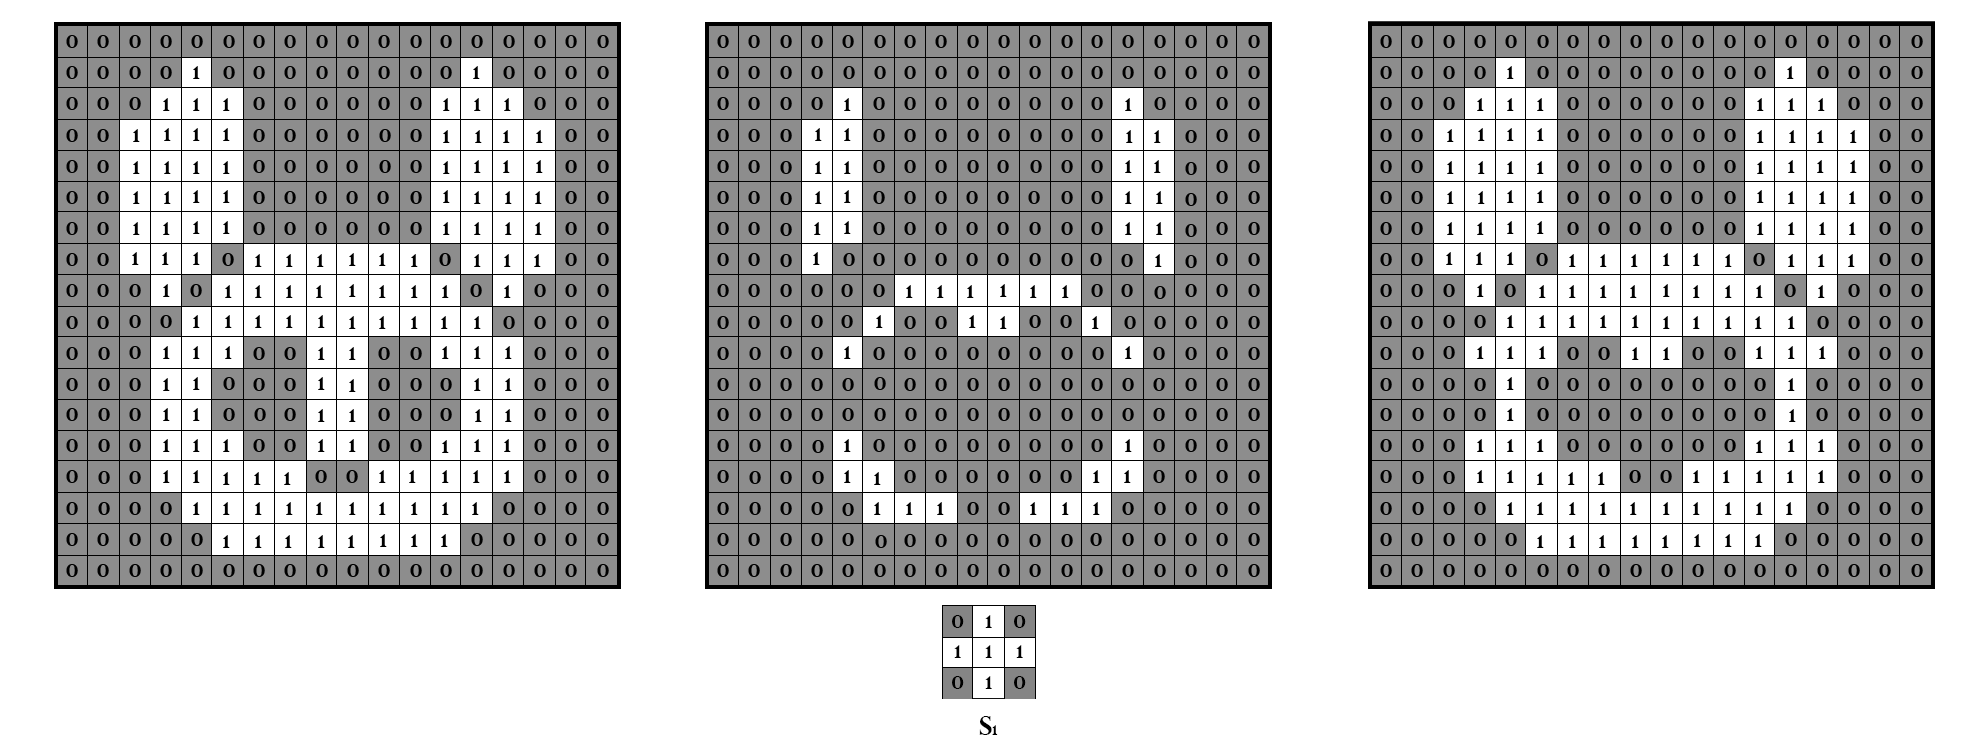
\includegraphics[width=1\textwidth]{Pictures/Theory/OpeningCirc.png}
\caption{Opening produced by a circular structured element.}
\label{fig:Opening}
\end{figure}

\subsubsection{Closing}
Another situation that often occurs when applying these methods comes from objects. When the size of the object is increased, but it's still important to constrain the measure as well as filling the holes of the objects, a good solution is to erode after the dilation. This is denoted \textit{closing} and uses eq. \ref{Closing}. As with the opening method, the size and shape of the kernel must be the same in order to obtain the desired result.

The effect of this operation can be seen on figure \ref{fig:Closing}: even though the holes are filled and the object maintains its original size, the noise of the background is still there. Therefore, it will be necessary to apply either closing or a BLOB analysis method to delete those small objects {BLOB analysis is described in \ref{blob}).
\begin{equation}
\begin{aligned}
{g(x,y)}={f(x,y)}\bullet{SE}=({f(x,y)}\oplus{SE})\ominus{SE}
\label{Closing}
	\end{aligned}
\end{equation}
It is also important to remember that the closing or opening methods should only be used one time on an image. Most of the holes of the image will be filled but the size of the object will be the original one. If these operations are applied a second time, the size of the final image will be decreased or increased respectively.

%%%%%%%%%%%%%%%%%%%%%%%%%%%%%%%%%%% IMAGE CLOSING %%%%%%%%%%%%%%%%%%%%%%%%%%%%%%%%%%%%
\begin{figure}[htbp]
\centering
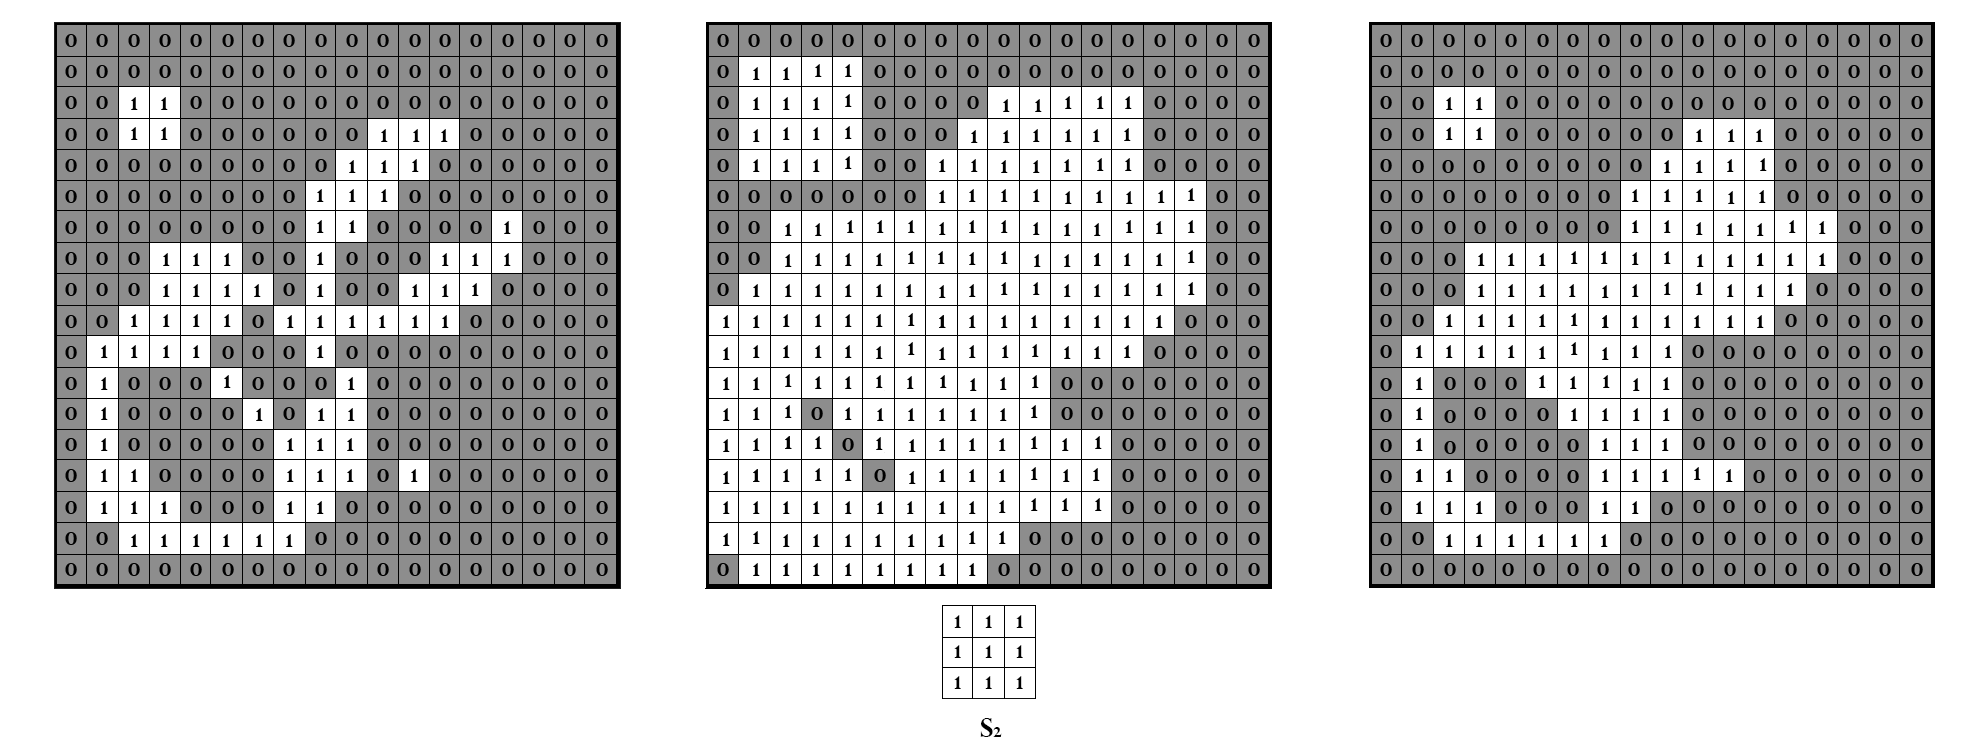
\includegraphics[width=1\textwidth]{Pictures/Theory/ClosingSq.png}
\caption{Closing produced by a squared structured element.}
\label{fig:Closing}
\end{figure}

\subsubsection{Boundary detection}
An alternative approach to the edge detection on binary images is the denoted \textit{boundary detection}. The performance of this operations is a compound of erosion and subtraction, hence the first operation will be eroding the object to get a smaller version of it and then subtract it to the original input image so as to get a final output image with the border of the object. The mathematical definition of these operations is
\begin{equation}
\begin{aligned}
{g(x,y)}={f(x,y)}-({f(x,y)}\ominus{SE})
\label{BoundDetec}
	\end{aligned}
\end{equation}
When the purpose of implementing these operations is to find the edges, it is important to remember to apply dilation or erosion before, to remove the noise of the image. The results can be seen on figure \ref{fig:Boundary} where the final result is a thin edge of the object.

%%%%%%%%%%%%%%%%%%%%%%%%%%%%%%%%%%% IMAGE SUBTRACTION %%%%%%%%%%%%%%%%%%%%%%%%%%%%%%%%%%%%
\begin{figure}[htbp]
\centering
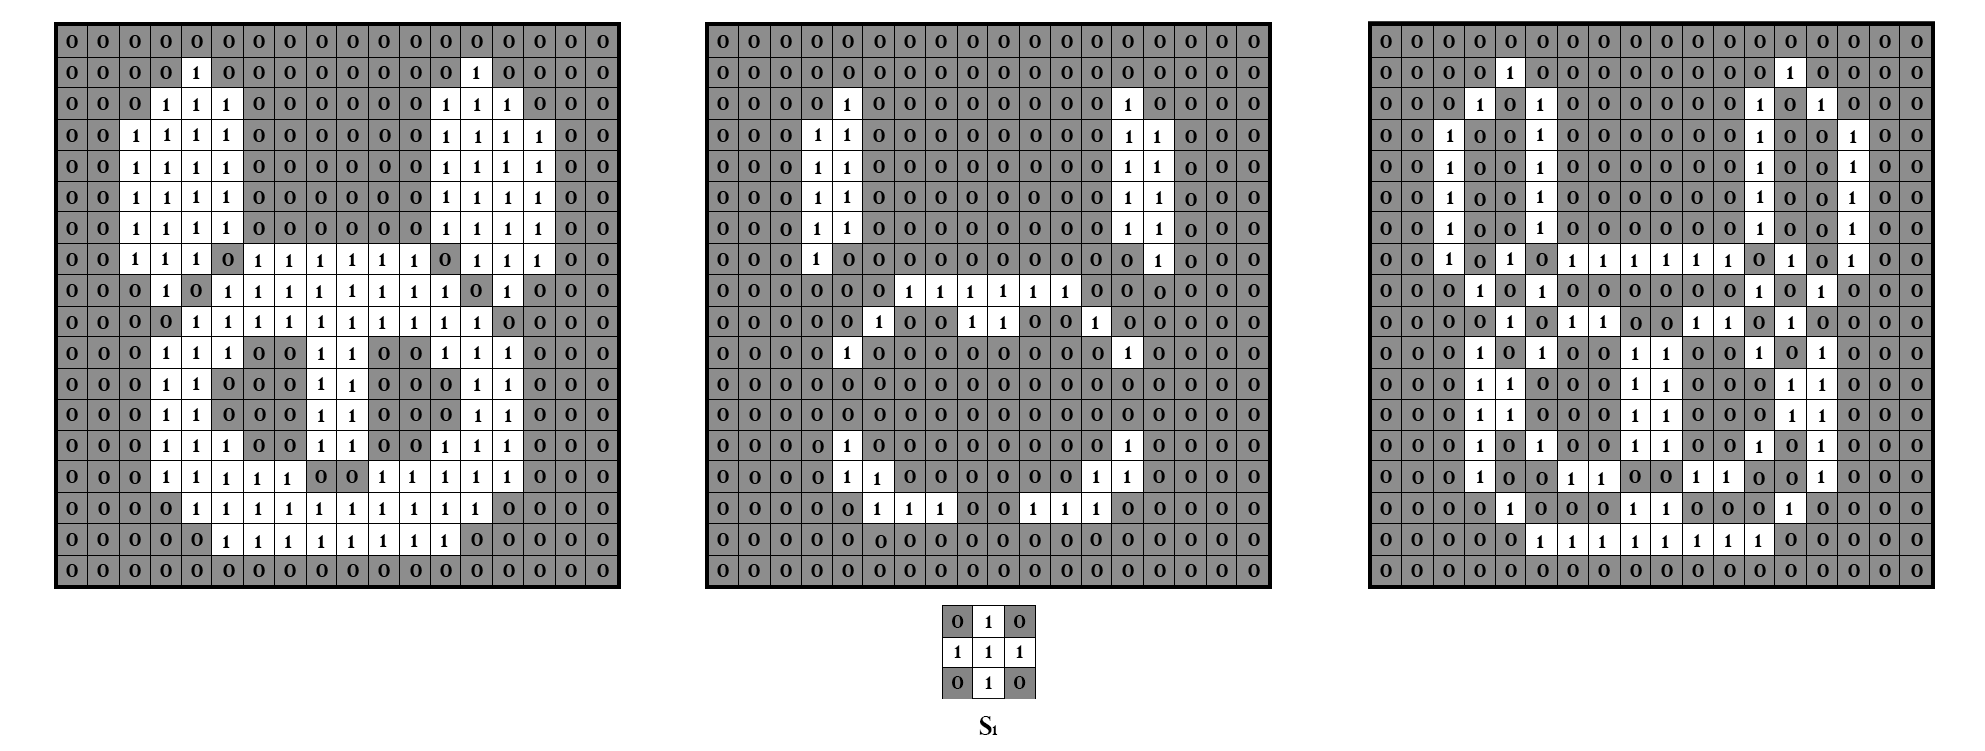
\includegraphics[width=1\textwidth]{Pictures/Theory/BoundaryEdges_circ.png}
\caption{Result of subtracting an eroded picture to the original one with a circular structured element.}
\label{fig:Boundary}
\end{figure}

\section{Region of interest (ROI)}
A common thinking when dealing with images is that the more pixels, the better quality. However, this is not always true. Since there are more pixels to loop through, it takes longer time to the program to analyze and process the data. The more pixels to process, the longer time requires the calculations to the program.

When working with video, it is important to maintain a stable framerate. The more information needed to process, the slower the overall program will be. One way to minimize the amount of data is to use what is called a \textit{region of interest} (ROI). As the name suggests, one should choose a specific region of the image that is of interest. This could for instance be the upper part of an image where heads are usually going to be. If one only wants to track or recognize a face, the rest of the body can be discarded.

A way to optimize the speed of the program is to decrease the data by using a region of interest. This region is usually enclosed in a rectangle and only the pixels inside this rectangle is being processed. That means that all the pixels outside of the ROI are ignored and unnecessary processing is prevented.

An example of how this could be used is taking a photo where only the head is of interest. This is illustrated on figure \ref{fig:Region of Interest}.

\begin{figure}[htbp] 
\centering 
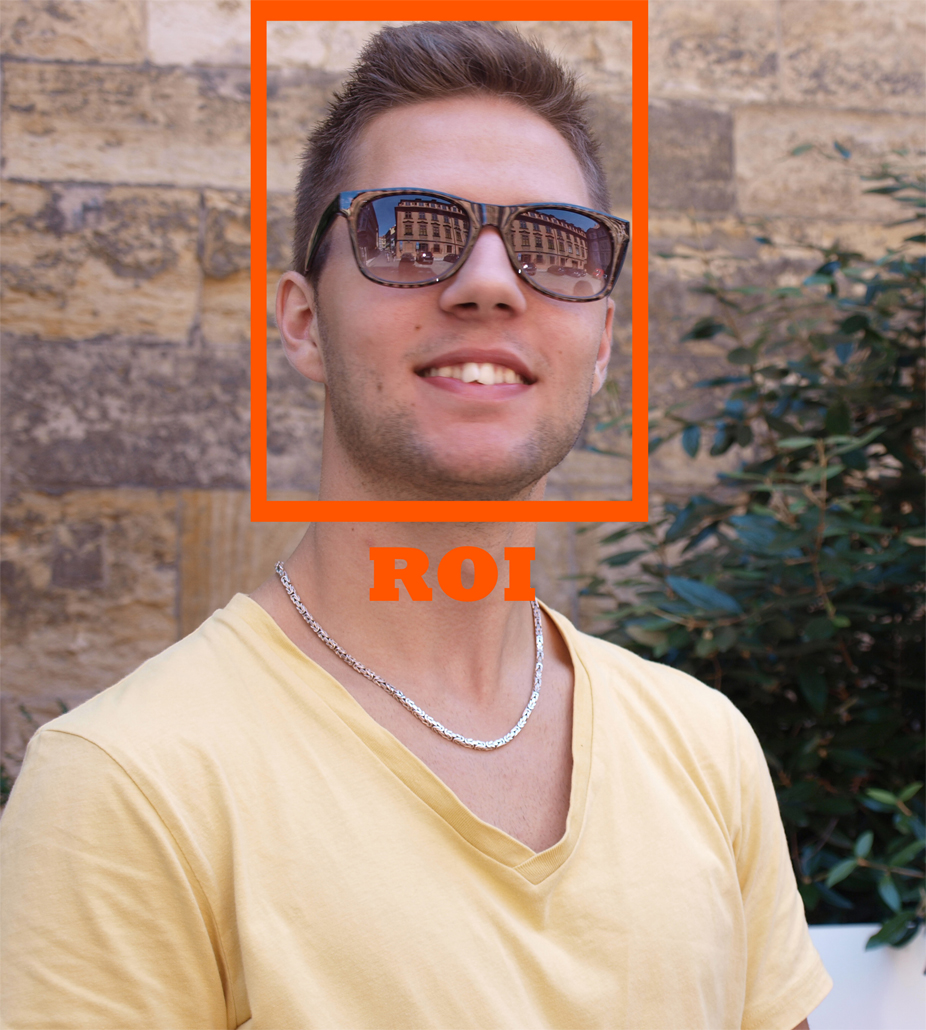
\includegraphics[width=0.5\textwidth]{Pictures/Theory/RegionOfInterest.jpg} 
\caption{If one needs to only track the face, a region of interest can be applied.} 
\label{fig:Region of Interest} 
\end{figure} 

\section{Noise reduction}
Noise reduction is very used in image processing, and is almost impossible to go around. When you e.g. threshold a picture then in most cases noise will appear. Either as small dots in the background or maybe small holes in the wanted area. Thankfully this noise can be reduced using different techniques. Two techniques that will be described further in this section is mean and median filters.\\
These two types of filters can be used to remove noise from the picture, and it is a question of what the output should show when picking technique.\\
A small description of how these two techniques works will be written in the subsection below.
\subsubsection{Mean filter}
One method of filtering is the mean filter. As the name implies a mean filter takes a input image, calculates the mean value of a given pixel and uses this as the output, a mean filter is a type of neighborhood processing. In practical application this means that the average of the input pixel and the surrounding pixels decides the value of the output pixel, see figure \ref{fig:neigh_pros}.

\begin{figure}[htbp] 
\centering 
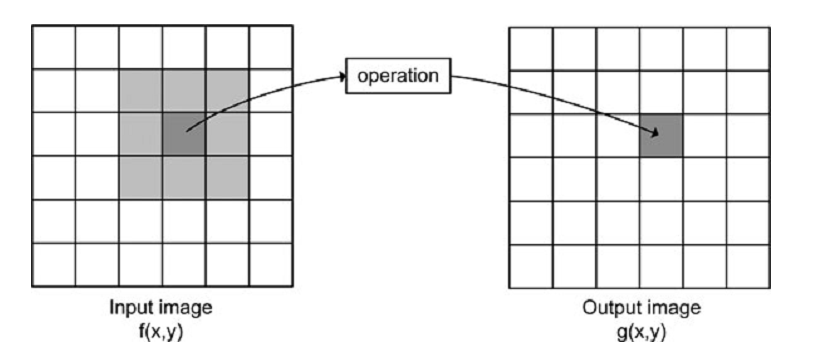
\includegraphics[width=0.5\textwidth]{Pictures/Theory/neighborhood_processing.png} 
\caption{Practical neighborhood processing. All the surrounding pixels contribute to the average value of the output.} 
\label{fig:neigh_pros} 
\end{figure}

The calculations that lie behind the average are simple:

\begin{equation}
	\begin{aligned}{
	\frac{\text{Sum of input $-$ and neighboring pixels}}{\text{number of pixels}}
	\label{Mean filter}	}
	\end{aligned}
\end{equation}

\subsubsection{Median filter}
Another method of filtering is the median filter. The median once again relies on the neighboring pixels. By indexing the input pixel along with its neighbors in a ordered list and choosing the middle value, i.e. the \textit{mean}, the output pixel is determined. In practical applications the algorithm required for a median filter can be broken down in to two steps: Creating a ordered list of the pixels and finding the mean value.

Taking out input pixels, $n_1$ through $n_9$ we first create a ordered list:


\begin{equation}
\begin{aligned}{
\text{Ordered list:}[n_1,n_2,n_3,n_4,n_5,n_6,n_7,n_8,n_9]
	\label{Order list of pixels.}}	
	\end{aligned}
\end{equation}

Then we find the median:

\begin{equation}
\begin{aligned}{
\text{Mean} [n_1,n_2,n_3,n_4,\textbf{$n_5$},n_6,n_7,n_8,n_9]
	\label{Finding the mean pixel.}}
	\end{aligned}
\end{equation}
\fxnote{Need to make this work the way it should.}

\section{Background subtraction}
A way to detect changes in a scene and extracting an object is using \textit{background subtraction}. As the name implies, it is done by subtracting the background from the scenery, so that only changes is shown.

In order to be able to use background subtraction efficiently, a controlled setup is required. The optimal setup is an indoor environment with controllable lights. The setup is important as the background should be static. Imagine if sunshine is let inside the room; then the light will change together with the sun's position, and changes will be seen everywhere and thereby producing noise that gives an inaccurate result.

It is not realistic that each pixel in the background keeps the exact same pixel value all the time. Therefore a threshold value is required - for two reasons. First of all to make the changes in the scene more distinct from the background, but also to have a threshold value in which the background may vary.

Therefore the following two questions have to be considered when doing background subtraction:
\begin{enumerate} 
	\item Is the background consistent? 
	\item Which threshold value would be optimal for making the picture binary, and distinct the changes from the background? 
\end{enumerate}

If the first point is false and the background is not consistent, there is a way to automatically update the backgrounds pixel values. The formula is shown in \ref{AutomaticBackground}.

\begin{equation}
	\begin{aligned}
  		r_{new}(x,y)=\alpha*r_{old}(x,y)+(1-\alpha)*f(x,y)
		\label{AutomaticBackground}  
 	\end{aligned}
\end{equation}  

Where $r(x,y)$ is the reference image, $f(x,y)$ is the current image, and $\alpha$ is the weighting factor. The weighting factor $\alpha$ defines how fast the reference image updates. A typical weighting factor value is  $\alpha = 0.95$ \citep{ip_book}.

Now that the background automatically updates, it is time to proceed to the next question: defining the threshold value.

To do this, it is necessary to check how much the backgrounds pixel values vary. This can be done by making a histogram for a group of pixels in the background and check the values after recording a few minutes. This should give an overview of how much the pixel values vary. Let's say that this procedure shows that an efficient threshold value is 20. This means that if a pixel in the background is of the intensity 80, then pixel values captured between the values $60-100$ will not make any changes, as it is seen as being the background. Pixels below 60 and above 100 will however be an object and highlighted. Another pixel in the background could have the intensity of 48 and the pixel values captured between $28-68$ would then be thought of as the background while values below 28 and above 68 would be seen as an object and be highlighted.

This type of threshold is a global threshold, which means that the threshold value is the same in every pixel in the scene \citep{ip_book}. Imagine a scene where only part of the picture is being affected by lights. Then a unique, local, threshold value for each pixel could be useful. This is possible using the eq. \ref{localthreshold}.

\begin{equation}
	\begin{aligned}
  		\ \text{Binary image} = \left\{ \begin{array}{ll}
         0, \quad &\text{if } Abs(g(x,y))<\beta * \sigma(x,y)\\
        255, \quad &\text{otherwise}.
        \end{array} \right . \ 
        \label{localthreshold}  
 	\end{aligned}
\end{equation} 

Where $\beta$ is the scaling factor, and $\sigma(x,y)$ is the standard deviation at the position $(x,y)$. Using this formula creates a local threshold.

When both questions have been considered, the background subtraction is ready to be applied. In every frame in the scene, each pixel will be checked for a possible change. If there is a change larger than what the threshold value allows, the pixel will be highlighted, revealing an object in the picture.

\section{BLOB analysis}\label{blob}
A common problem when dealing with images is to determine if the image data contains a particular object or shape. The term \textit{BLOB} is an acronym for Binary Large Object and refers to a region of connected pixels in a binary image. This technique is used to extract meaningful information from images. This is achieved by separating the pixels in points or regions that differ in properties, like brightness or color changes (i.e., their value), and classifying them into one of two categories: the foreground (pixels with a non-zero value) and the background (pixels with values equal to zero).
Therefore, BLOB analysis will be split in three main steps: \textit{extraction} of the BLOBs, \textit{representation} of the BLOBs and, lastly, \textit{classification} of the BLOBs to know which ones belong to the expected type \citep{ip_book}.

\subsection{BLOB extraction}
To isolate BLOBs in a binary image, we need to know if two pixels are connected or not. This is done by applying algorithms that will help to determine the connectivity of the pixels, but also the number of BLOBs contained in an image. The most commonly-used kernels in BLOB extraction are the 8-connected and the 4-connected kernels \citep{ip_book}. The 8-connected kernel is more accurate, but also requires more computations and therefore needs more time to process the image.

\subsubsection{Grass-fire algorithm}
One of these connected component labelling algorithms is the \textit{recursive grass-fire algorithm}, used to erode images, but also to track the pixels locations to create a region.
To explain this algorithm, we will use both 8-connectivity and 4-connectivity kernels to illustrate how these choices can affect to the final result.

\begin{figure}[htbp]
\centering
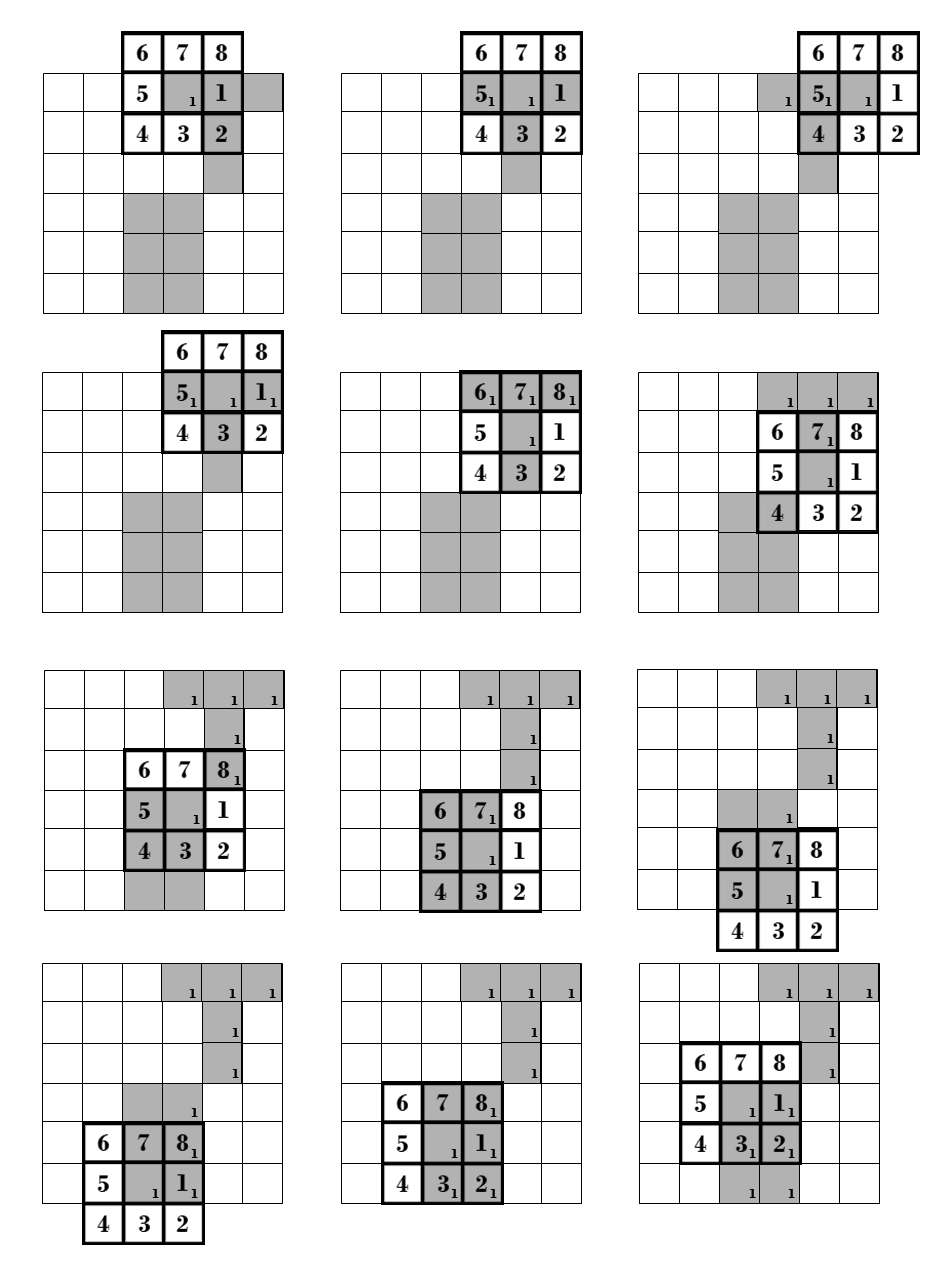
\includegraphics[width=0.8\textwidth]{Pictures/Theory/8connec_kernel.png}
\caption{8-connectivity labelling kernel detects a single object. Inspired by \citep{ip_book}.}
\label{fig:8connecK}
\end{figure}

As shown in figure \ref{fig:8connecK}, the grass-fire algorithm scans the entire image from the upper-left corner to the right bottom, row by row. When the kernel encounters a non-zero pixel value, it centers on it and "burns" the center pixel. Then the algorithm looks in the possible directions around that pixel to check if those pixels are connected to the previous one and therefore, together make out an object. The way the algorithm will do this will depend on the connectivity used (for a 8-connected kernel, the algorithm will look in 8 directions, but for the 4-connected kernel, the algorithm will look in 4 directions).

Whenever it finds an object, the algorithm labels the pixel in the output image and then burns that pixel on the input image, in order to turn it into a zero and ensure that the pixel will not be part of a new grassfire.

The algorithm now looks to the possible directions around that pixel, starting with the pixel on the right. This process is represented on figure \ref{fig:8connecK}. Once it finds a non-zero pixel value, the algorithm once again centers its attention on it and repeats the process, labelling the pixel with the number of the previous one. At the end of that row the algorithm will check the surrounding pixels on the row below. If a non-zero pixel value is found, the algorithm will continue the process of burning and labelling pixels, otherwise the algorithm will start its way back to the beginning checking the surrounding pixels one by one to verify that it has checked all the possible directions and non-zero pixels values.

Comparing figures \ref{fig:8connecK} and \ref{fig:4connecK}, we can realize how the choice of a certain kernel will affect the final result of the algorithm using the same picture. Although the 8-connected kernel is more accurate it seems to be unable to separate the different objects as intended in this particular case, whereas the 4-connectivity kernel finds the different objects performing less operations.

\begin{figure}[htbp]
\centering
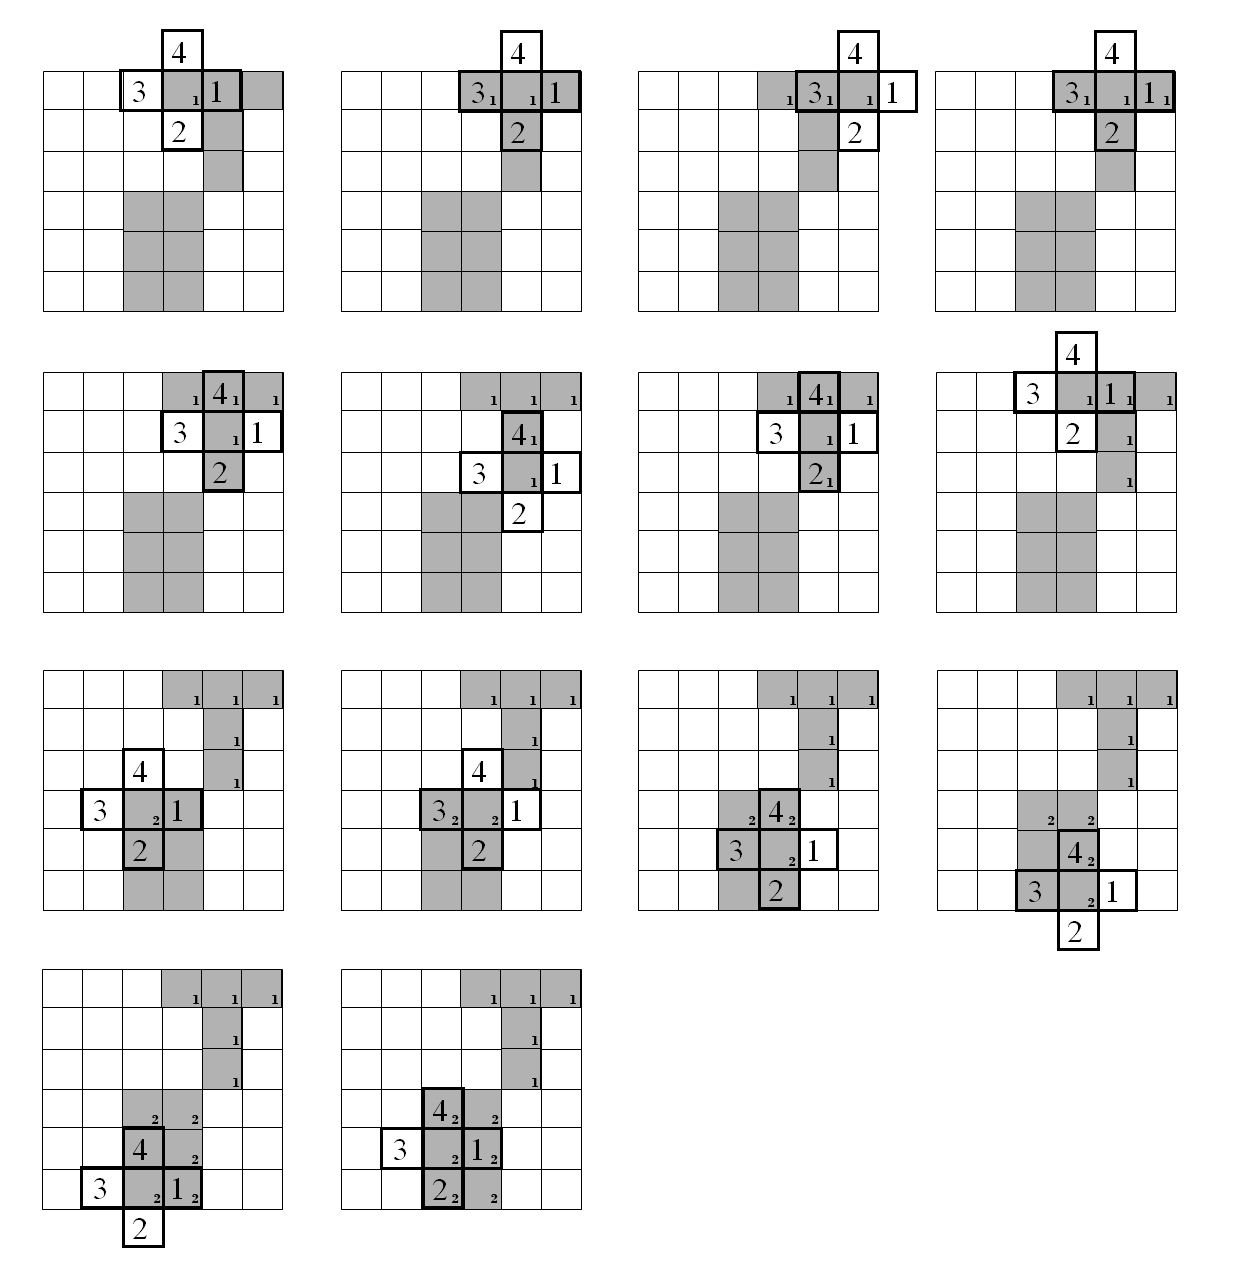
\includegraphics[width=0.75\textwidth]{Pictures/Theory/4connec_kernel.png}
\caption{4 connectivity labelling kernel detects two objects. Inspired by \citep{ip_book}.}
\label{fig:4connecK}
\end{figure}

\subsection{BLOB representation}
The classification of the BLOBs is made by creating a prototype model of the object that we are looking for in order to state the features the BLOB should contain, and the deviations that would be acceptable. This process consists of two steps: determining the features of the BLOB; and matching the features with the prototype to determine if they are part of the type that we were looking for.

This means that a few features like the area, the perimeter and the circularity will be calculated \citep{ip_book}.
\subsubsection{The features}

%%% Maybe delete this section? - Gustav, Dec 14 %%%
%%% Maybe delete this section? - Gustav, Dec 14 %%%
%%% Maybe delete this section? - Gustav, Dec 14 %%%

\begin{itemize}
\item \textbf{Area}
The importance of calculating features like the area of a BLOB is well understood if we keep in mind that one of the first steps while classifying the detected objects is to delete those that are bigger or smaller than the prototype. One way of doing this is by calculating the area of the BLOB.
\item \textbf{Bounding box and bounding circle}
Both bounding box and bounding circle are methods that operate in a similar way, as the particularity of these features is to find the minimum box or circle that can enclose the BLOB. The difference between these two, besides the shape, is the way they operate. While the bounding box is the minimum rectangle and operates by finding four pixels; $x_max$, $x_min$, $y_max$ and $y_min$, which represent the minimum and maximum X and Y values than can create a box that encompasses the BLOB. The bounding circle is the minimum circle and needs to find first the center of the BLOB.
\item \textbf{Convex hull}
The minimum convex polygon that contains the BLOB can be described as wrapping a piece of strings tightly around the BLOB. Starting from the topmost pixel of the BLOB and searching to the right along a horizontal line and in a clockwise motion till it finds a BLOB pixel and creates the first side of the polygon.
\item \textbf{Bounding box ratio}
This is the height of the bounding box divided by the width, indicating the height-to-width ratio of the BLOB.
\item \textbf{Compactness}
The compactness of a BLOB is the ratio of the BLOBs area to the ratio of the bounding box. See eq. \ref{compact}.
\begin{equation}
	\begin{aligned}
	\text{Compactness}=\displaystyle\frac{BLOB's Area}{width\cdot{height}}
	\label{compact}
	\end{aligned}
\end{equation}

\item \textbf{Center of mass}
In physics, the center of mass is the unique point where the mass of an object is equally distributed. The common example to explain this would be the place where you have to place your finger on an object in order to have it balanced.

The distribution of mass is balanced around the center of mass and the average of the weighted position coordinates of the distributed mass defines its coordinates. On a binary image, this center will be the average X and Y positions of the object on the image.

Its coordinates can be found using eq. \ref{centermass}.

\begin{equation}
	\begin{aligned}
  		\ \text{Center of Mass} = \left\{ \begin{array}{ll}
         x_{c}=\displaystyle\frac{1}{N} \displaystyle\sum_{i=1}^N x_{i}\\
         y_{c}=\displaystyle\frac{1}{N} \displaystyle\sum_{i=1}^N y_{i}
        \end{array} \right . \ 
\label{centermass} 	
 	\end{aligned}
\end{equation} 


Where N is the number of pixels in the BLOB and $x_i$ and $y_i$ are the coordinates of each single pixel inside that BLOB. In some situation where we will need to calculate the center of mass of an object with annexed parts, a median filter or an erosion before using the previous formula would be appropriate.

\item \textbf{Center of the bounding box}
As the bounding box is a rectangle that surrounds the BLOB, the center of the bounding box is an approximation of the center of mass and can be found with eq. \ref{BoundingBoxCenterX} and \ref{BoundingBoxCenterY}.

\begin{equation}
	\begin{aligned}	x_{bb}=x_{min}+\displaystyle\frac{x_{max}-x_{min}}{2}=x_{min}+\displaystyle\frac{x_{max}}{2}-\displaystyle\frac{x_{min}}{2}=\displaystyle\frac{x_{min}+x_{max}}{2}
	\label{BoundingBoxCenterX}
	\end{aligned}
\end{equation}

\begin{equation}	
	\begin{aligned}
	y_{bb}=y_{min}+\displaystyle\frac{y_{max}-y_{min}}{2}=y_{min}+\displaystyle\frac{y_{max}}{2}-\displaystyle\frac{y_{min}}{2}=\displaystyle\frac{y_{min}+y_{max}}{2}
	\label{BoundingBoxCenterY}
	\end{aligned}
\end{equation}


\item \textbf{Perimeter}
Scanning along the border of the BLOB and summing the pixels, we obtain the length of the contour of the BLOB. In image processing, this could be done by using morphology techniques like erosion to get a smaller version of the object and then subtracting this to the input image in order to get the edges.
\item \textbf{Circularity}
Circularity is a common shape-factor that depends on the perimeter and the area. There are several ways to define how circular an object can be, but usually applying the ratio to get a value lower or equal to 1 will indicate how circular the BLOB is, where 1 is a complete circle. See eq. \ref{Circularity}.


\begin{equation}	
	\begin{aligned}
	{Circularity}=\displaystyle\frac{BLOB's \;\; Perimeter}{2 \; \sqrt{\mathstrut \: \pi \: \cdot \: {BLOB's \;\; Area}}}
	\label{Circularity}
	\end{aligned}
\end{equation}


After all the features are extracted, a binary object can be defined by its feature values that would be stored into a feature vector in order to have a list where to start the BLOB classification.
\end{itemize}

% IMAGE WITH OBJECTS AND TABLE WITH DATA

\begin{figure}[ht]
\begin{minipage}[b]{0.45\linewidth}
\centering
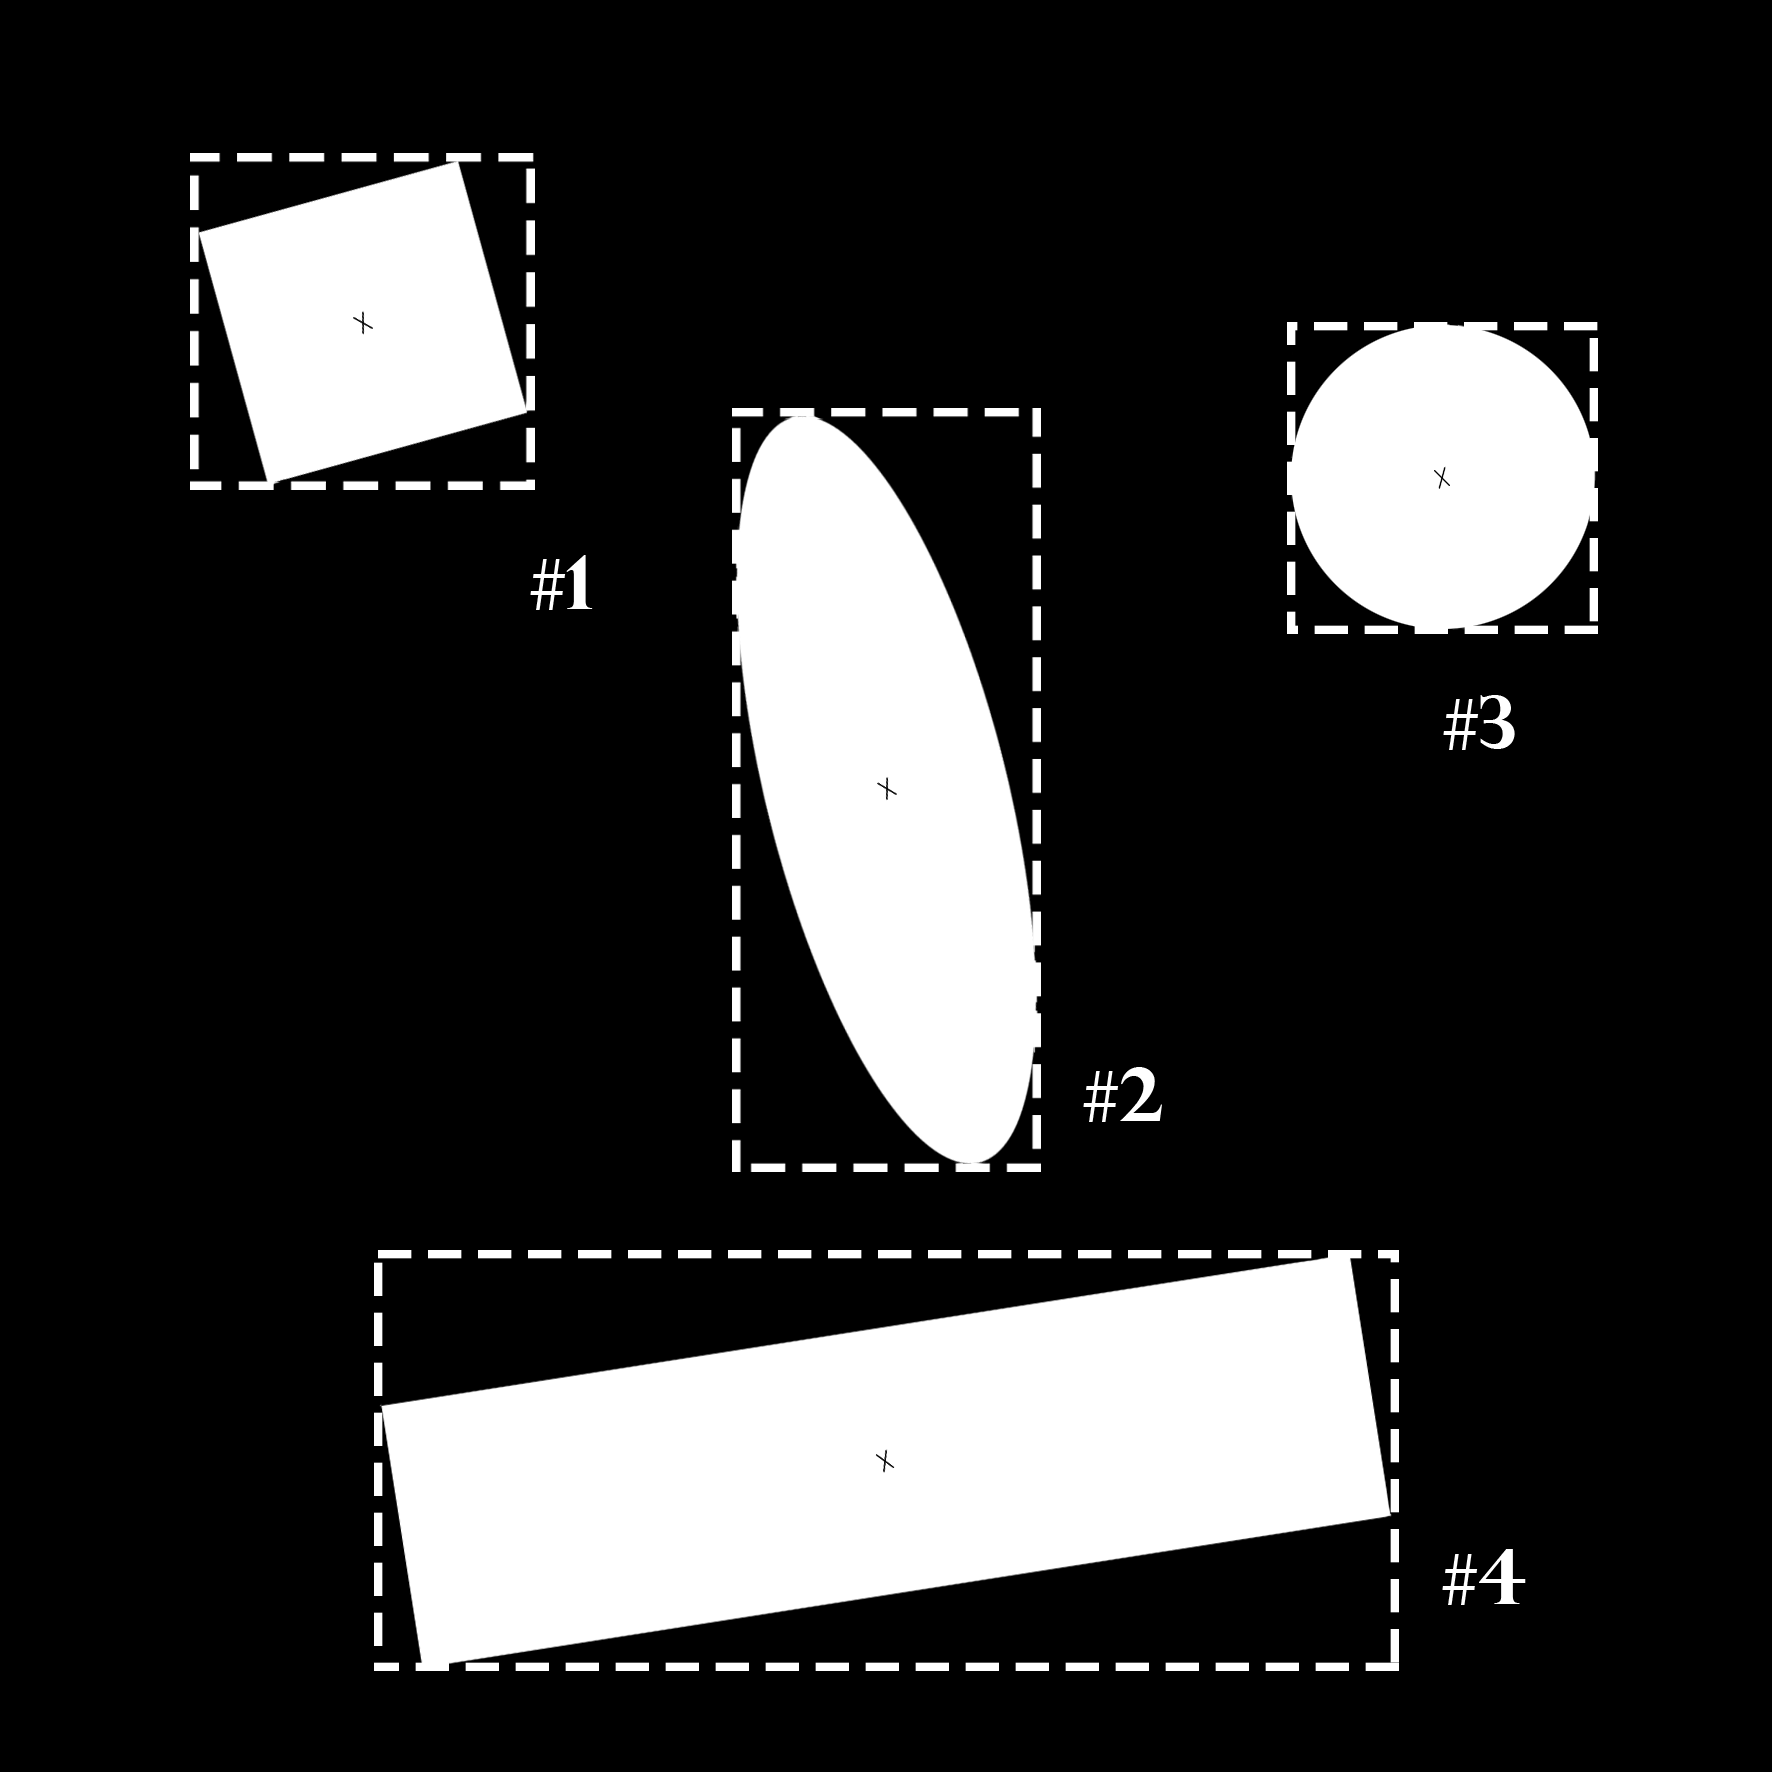
\includegraphics[width=1\textwidth]{Pictures/Theory/binary_image.png}
\end{minipage}
\hspace{0.5cm}	
\begin{minipage}[b]{0.45\linewidth}
\centering
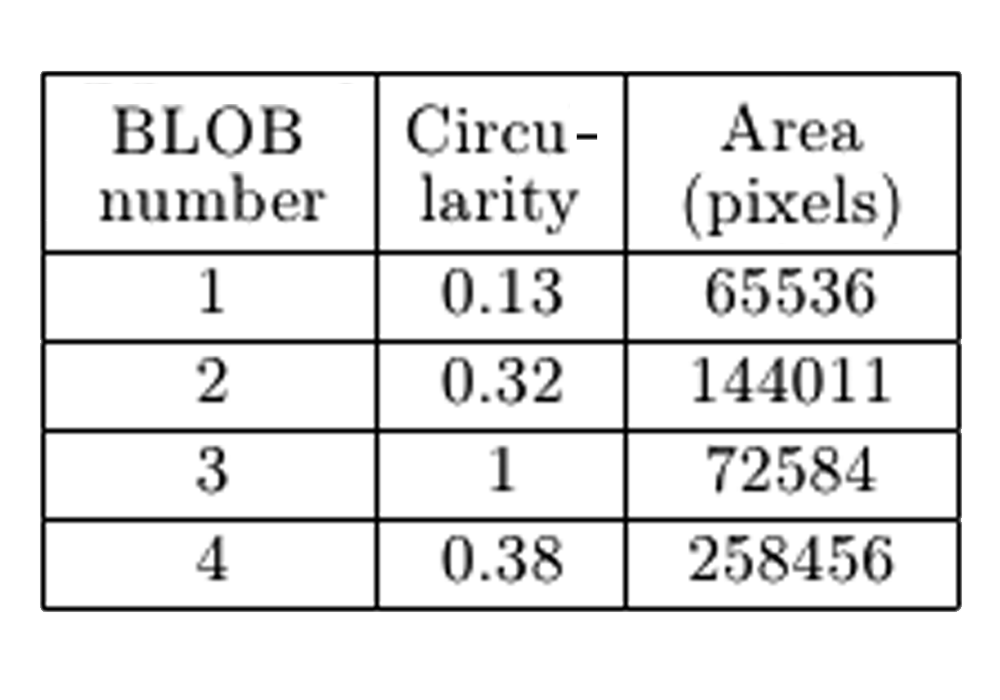
\includegraphics[width=1\textwidth]{Pictures/Theory/binary_image_table.png}
\end{minipage}
\label{fig:BinaryIm}
\caption{Binary image with a bounding box and the center-of-mass. The table shows two other features that can be calculated: the perimeter and the area. Inspired by \citep{ip_book}.}
\end{figure}

%%%%%%%%%%%%%%%%%%%%%%%%%%%%%%%%%%%%%%%%%%%%%%%%%%%%%%%%%%%%%%%%%%%%%%%%%%%%%%%%

\subsection{BLOB classification}
Once we have extracted and represented each object on the binary image by its features, we need to determine the minimum characteristics that the object has to comply to, in order for it to be selected. For this reason we will define a \textit{prototype model} based on ideal measurements that is used as a reference to which the extracted values are compared. As the real object will not be perfect, a deviation is needed to create a tolerance range.

Using two features like the circularity and the area, we will create a frame, also known as a \textit{box classifier}, and every object belonging to that \textit{feature space}, also know as \textit{decision region}, will then be understood as a desired object.

Another way to achieve this would be to create a \textit{statistical classifier} using means and variances of the features, where the task would be to measure the distance between a new feature vector and the prototype. The smaller the distance between those two, the more likely the object will be part of the same type. But before getting to this point, we need to threshold the distance and consequently have a binary decision region like the box classifier. This time, the region will not be a rectangle but an ellipse, and is commonly known as the \textit{weighted Euclidean distance}, as shown in eq. \ref{Euclidean}.

\begin{equation}	
	\begin{aligned}
{WED(\vec{f}_{i} \; , \: prototype)} \: = \: \sqrt{\mathstrut \:  \displaystyle\frac{(f_{i}(cir) \: - \: mean(cir))^2}{variance(cir)} \: + \: \displaystyle\frac{(f_{i}(area) \: - \: mean(area))^2}{variance(area)}}
\label{Euclidean}
	\end{aligned}
\end{equation}

The final result is the distance between the vector {$\vec{f}_{i}$} and the prototype. The values of {$f_{i}(cir)$} and {$f_{i}(area)$} correspond to the circularity and the area of every object found on the binary image. For an image with a number of N different features, the result would be obtained by eq. \ref{Euclidean1}.

\begin{equation}	
	\begin{aligned}
{WED(\vec{f}_{i} \; , \: prototype)} \: = \: \displaystyle\sum_{i=1}^N \: \: \sqrt{\mathstrut \:  \displaystyle\frac{(f_{i}(m_{j}) \: - \: mean(m_{j}))^2}{variance(m_{j})}}
\label{Euclidean1}
	\end{aligned}
\end{equation}

Where {$m_{j}$} is the {$jth$} feature. When the variances of the features are the same all along the list of values, we can ignore it and calculate the Euclidean distance (ED), where the region is a circle in 2D, see eq. \ref{Euclidean2}.

\begin{equation}	
	\begin{aligned}
{ED(\vec{f}_{i} \; , \: prototype)} \: = \: \displaystyle\sum_{i=1}^N \: \sqrt{\mathstrut (f_{i}(m{j}) - mean(m_{j}))^2}
\label{Euclidean2}
	\end{aligned}
\end{equation}

But before we can calculate the distances, we need to normalize the values to the same scale and interval.

Therefore, the area would be done by \ref{NormArea}.
\begin{equation}	
	\begin{aligned}
{Area \: feature} \: = \: min \begin{Bmatrix} \displaystyle\frac{Area\:of\:BLOB}{Area\:of\:Model}, & \displaystyle\frac{Area\:of\:Model}{Area\:of\:BLOB}\end{Bmatrix}
\label{NormArea}
	\end{aligned}
\end{equation}

The circularity can also be normalized in the same, eq. \ref{NormCirc}.

\begin{equation}	
	\begin{aligned}
{Circularity \: feature} \: = \: min \begin{Bmatrix} {Circularity}, & \displaystyle\frac{1}{Circularity}\end{Bmatrix}
\label{NormCirc}
	\end{aligned}
\end{equation}